\documentclass[a4paper]{article}

\usepackage{adjustbox}
\usepackage{algorithm}
\usepackage{algorithmic}
\usepackage{amsmath}
\usepackage{amssymb}
\usepackage{amsthm}
\usepackage{amsfonts}
\usepackage{afterpage}
\usepackage{blindtext}
\usepackage[font=footnotesize,labelfont=bf]{caption}
\usepackage{hyperref}
\usepackage[english]{babel}
\usepackage{bbm}
\usepackage{bigints}
\usepackage{bm}
\usepackage{cite}
\usepackage{color}
\usepackage{float}
\usepackage[left=2cm,right=2cm,top=2cm,bottom=2cm]{geometry}
\usepackage{graphicx}
\usepackage[utf8]{inputenc}
\usepackage{mathtools}
\usepackage{mdframed}
\usepackage{pgfplots} 
\usepackage{subfigure}
\usepackage{stmaryrd}
\usepackage{textcomp}
\usepackage{tikz}
\usepackage{url}
\renewcommand{\proofname}{Proof}
\theoremstyle{plain}
\newtheorem{monTheoNumrote}{Théorème}[section] % Environnement numéroté en fonction de la section
\newtheorem*{monTheoNonNumerote}{Théorème}  % Environnement non numéroté
\newtheorem{The}{Theorem}[section]
\newtheorem*{The*}{Theorem}
\newtheorem{Prop}{Proposition}[section]
\newtheorem*{Prop*}{Proposition} 
\newtheorem{Cor}{Corollary}[section]
\newtheorem*{Cor*}{Corollary}
\newtheorem{Conj}{Conjecture}[section]
\newtheorem{Lem}{Lemma}[section]
\renewcommand{\qed}{\unskip\nobreak\quad\qedsymbol}%
\numberwithin{equation}{section} % Numérote les équations section.numéro.
\theoremstyle{definition}
\newtheorem{Def}{Definition}[section]
\newtheorem{Rem}{Remark}[section]
\newtheorem*{Rem*}{Remark}
\newtheorem*{Lem*}{Lemma}
\newtheorem{Que}{Question}
\newcommand{\enstq}[2]{\left\{#1\mathrel{}\middle|\mathrel{}#2\right\}}
\newcommand{\Lp}[2]{L^#1(#2)}
\newcommand{\Sob}[3]{W^{#1,#2}(#3)}
\newcommand{\Rd}[0]{\mathbb{R}^d}
\newcommand{\RN}[0]{\mathbb{R}^N}
\newcommand{\Rn}[0]{\mathbb{R}^n}
\newcommand{\norm}[1]{\left\|#1\right\|}
\newcommand{\sinc}[0]{\textup{sinc}}
\newcommand{\functionDef}[5]{\begin{array}{lllll}
#1 & : & #2 & \longrightarrow & #3 \\
 & & #4 & \longmapsto &\displaystyle #5 \\
\end{array}}
\newcommand{\Theautorefname}{Theorem}
\newcommand{\Propautorefname}{Proposition}
\newcommand{\Corautorefname}{Corollary}
\newcommand{\Lemautorefname}{Lemma}
\newcommand{\Defautorefname}{Definition}
\newcommand{\N}{\mathbb{N}}
\newcommand{\Z}{\mathbb{Z}}
\newcommand{\D}{\mathbb{D}}
\newcommand{\R}{\mathbb{R}}
\newcommand{\A}{\mathcal{A}_{a,b}}
\newcommand{\Crad}{C^\infty_{c,rad}(B)}
\newcommand{\Lrad}{L^2_{rad}(B)}
\newcommand{\Lradab}{L^2_{rad}(\mathcal{A}_{a,b})}
\newcommand{\duality}[2]{\left\langle #1,#2\right\rangle}
\newcommand{\Hrad}{H^1_{rad}(B)}
\newcommand{\Hzrad}{H^1_{0,rad}(B)}
\newcommand{\rmin}{\delta_{\min}}
\newcommand{\rmax}{\delta_{\max}}
\newcommand{\corr}{\gamma}
\newcommand{\question}[1]{\begin{Que} \ 
#1
\end{Que}}
\newcommand{\abs}[1]{\left\lvert #1 \right\rvert}
\newcommand{\CL}[2]{\textup{CL}\left(\enstq{#1}{#2}\right)}
\newcommand{\Script}[1]{`\texttt{#1}`}
\newcommand{\espace}{\text{ }\qquad} 
\newcommand{\loc}{\text{loc}}
\newcommand{\SL}{\textup{SL}\hspace{1.5pt}}
\newcommand{\DL}{\textup{DL}\hspace{1.5pt}}
\newcommand{\fp}{\underset{\varepsilon \to 0}{\textup{f.p.}}}
\newcommand{\scalProd}[2]{\left(#1|#2\right)}
\newcommand{\toDo}[1]{{\color{red}#1}}
\newcommand{\bs}[1]{\boldsymbol{#1}}
\newcommand{\varInRange}[4]{(#1_{#2})_{#3 \leq #2 \leq #4}}
\newcommand{\from}{\colon}
\newcommand{\Cinf}{C^{\infty}}
\newcommand{\isdef}{\mathrel{\mathop:}=}
\newcommand{\defis}{=\mathrel{\mathop:}}

\renewcommand{\algorithmicrequire}{\textbf{Inputs:}}
\renewcommand{\algorithmicensure}{\textbf{Outputs:}}

\pgfplotsset{compat=1.13}
\usepackage{todonotes}
\pdfminorversion=7
\title{New preconditioners for Laplace and Helmholtz integral equations on open curves: \\
	\vspace{0,5cm}
	\begin{Large}
		I. Theoretical framework and numerical results. 
	\end{Large}}
\author{Fran\c{c}ois Alouges and Martin Averseng\footnote{CMAP, Ecole polytechnique, Route de Saclay, 91128 Palaiseau Cedex.}}
\begin{document}
\maketitle

\begin{abstract}
Studying wave scattering problems in 2D by open arcs leads to ill-conditioned systems. This is partly due to the singular behavior
of the solutions near the edges of the arc. We introduce two new preconditioners to tackle this problem either with Dirichlet or Neumann 
boundary data, that take the form of square roots of local operators. We introduce an adapted analytical setting to analyze them and 
demonstrate the efficiency of this method on several numerical examples. A complete suitable pseudo-differential calculus for the
complete study of such operators is postponed to the second part of this work.
\end{abstract}

\section{Introduction}

The problem of preconditionning the linear systems coming from the discretization of first kind integral equations
has received considerable attention since two decades. Among the possible strategies are the so-called pseudo-differential 
preconditionners \cite{alouges2007stable,alouges2005new,antoine2007generalized,christiansen2002preconditioner,hiptmair2014mesh,Steinbach98}. 
Roughly speaking, if the original problem is written in the abstract form
\begin{equation}
	\mathcal{L}u=f\,,
	\label{eq1}
\end{equation}
where $\mathcal{L}$ is a linear operator, the strategy consists in left multiplying equation (\ref{eq1}) by an operator $\mathcal{K}$ and solve
\begin{equation}
	\mathcal{K}\mathcal{L}u=\mathcal{K}f\,.	
\end{equation}
Now, if $\mathcal{K}\mathcal{L}$ is a compact perturbation of the identity, the condition number of the discretized underlying linear system 
becomes independent of the mesh size, enabling the efficient use of iterative methods such as GMRES \cite{saad1986gmres}. This is in particular the 
case when $\mathcal{K}$ is a parametrix of $\mathcal{L}$, which is usually proven using tools from pseudo-differential calculus 
\cite{steinbach1998construction}.

Several strategies, depending on the problem to solve (e.g. Helmholtz or Maxwell equations) have been studied in the literature to propose such 
operators $\mathcal{K}$, that often turn out to be very effective in practice, when numerical applications are considered. Among those, we would 
like to emphasize the viewpoint first proposed in \cite{alouges2005new,alouges2007stable}, where, for Helmholtz equation, the authors consider 
integral formulations of the problem that involve the Dirichlet-Neumann map $DN$ which leads to well-conditioned systems after discretization. 
Combined with the approximation of $DN$ proposed first in \cite{antoine2007generalized} under the form of the square root operator
\begin{equation}
DN \sim \sqrt{-\Delta_\Gamma -k^2}\,,
\end{equation}
where $\Delta_\Gamma$ stands for the Laplacian operator on the surface $\Gamma$, the method (called GCSIE) yields a very impressive 
reduction of the number of iterations. 

However, all the preceding results and theories are limited to smooth surfaces $\Gamma$ and very little is known when the integral equation 
is posed on non-smooth domains, such as domains with corners (in 2D), wedges or conical points (in 3D). One of the reasons might be the 
fact that pseudo-differential calculus is difficult to generalize on such manifolds and the existing theories such as the ones presented in e.g. 
\cite{melrose,schulze1,schulze2} do not seem to be adequate for the analysis of such problems.

Nevertheless, attempts to precondition the integral equations that come from the discretization of single-layer or double-layer potentials 
for Laplace equation on singular domains has started a few years ago \cite{bruno2012second,hiptmair2017closed,jerez2012explicit,
hiptmair2014mesh,ramaciotti2017some} in dimension 2 or 3, but for very particular domains such as a straight and then curved segments 
in 2D and a unit disc in 3D. In most of these works, weighted versions of the usual integral operators are introduced, which enjoy better 
mapping properties than the standard operators, and the analysis is obtained ``by hand'' without any explicit use of pseudo-differential calculus. 

The aim of this paper and the forthcoming \cite{averseng} is twofold. Here we describe an analytical framework and a Galerkin method suited to the inversion of these weighted operators, with optimal rates of convergence. On the other hand, we build efficient preconditioners for the linear systems arising from the previous Galerkin method. The complete description and analysis of the method is postponed to \cite{averseng} and we instead focus in 
the present paper on the description and the numerical implementation. Preliminary analytical results, that show the optimality of the approach
for Laplace problems, are nevertheless included here.
	
The paper is organized as follows: in the first section, we introduce the notations and the usual boundary integral operators on an open curve. 
In the second section, we treat the case of the Laplace equation, where it is possible to derive explicit inverses of the weighted layer potentials 
in terms of square roots of local operators. We then generalize our results to non-zero frequency and non-flat arc in the third section. In the last 
section, we show the efficiency of this approach on several numerical examples. 

%%%%%%%%%%%%%%%%%%%%%%%%%%%%

\section{The scattering problem outside an open curve}

Let $\Gamma$ be a smooth non-intersecting bounded open curve in $\mathbb{R}^2$, and let $k \geq 0$ the wave number. We seek a solution 
of the Helmholtz equation
\begin{equation}
	-\Delta u - k^2 u = 0,  \text{ in } \R^2 \setminus \Gamma
	\label{Helmholtz}
\end{equation}
when one considers furthermore Dirichlet or Neumann boundary conditions, namely
\begin{equation}
	u = u_D, \text{ on } \Gamma
\label{Dirichlet}
\end{equation}
or
\begin{equation} 
	\dfrac{\partial u}{\partial n} = u_N  \text{ on } \Gamma 
\label{Neumann}
\end{equation}
respectively. In order for the problem to be well posed, we also need to impose suitable decay at infinity, given by the Sommerfeld condition
\begin{equation}
	\dfrac{\partial u}{\partial r} - iku = o\left(\frac{1}{\sqrt{r}}\right)
\label{Sommerfeld}
\end{equation}
with $r=|x|$ for $x\in \mathbb{R}^2$ .
Notice that in equation \eqref{Neumann}, $n$ stands for a smooth unit vector normal to $\Gamma$. 

\noindent Existence and uniqueness of solutions to the previous problems are guaranteed by the following theorem.
\begin{theorem}
\cite{stephan1984augmented,wendland1990hypersingular,monch1996numerical}. Assume $u_D \in H^{1/2}(\Gamma)$, and $u_N \in H^{-1/2}(\Gamma)$. 
Then problems (\ref{Helmholtz},\ref{Dirichlet},\ref{Sommerfeld}) and (\ref{Helmholtz},\ref{Neumann},\ref{Sommerfeld}) both possess a unique solution 
$u \in H^1_\textup{loc}(\R^2 \setminus \Gamma)$, which is of class $C^{\infty}$ outside $\Gamma$. \end{theorem}
\noindent For the definition of Sobolev spaces on smooth open curves, we follow
\cite{mclean2000strongly} by considering any smooth closed curve $\tilde{\Gamma}$ containing $\Gamma$, and defining 
\[H^s(\Gamma) = \enstq{U_{|\Gamma}}{ U \in H^s(\tilde{\Gamma}) }.\]
This definition does not depend on the particular choice of the closed curve $\tilde{\Gamma}$ containing $\Gamma$. Moreover, we also define
\[\tilde{H}^s(\Gamma) = \enstq{u \in H^s(\Gamma)}{\tilde{u} \in H^s(\tilde{\Gamma})}\]
where $\tilde{u}$ denotes the extension by zero of $u$ on $\tilde{\Gamma}$.

The solution to (\ref{Helmholtz},\ref{Dirichlet},\ref{Sommerfeld}) and (\ref{Helmholtz},\ref{Neumann},\ref{Sommerfeld}) can be furthermore expressed in 
terms of the Green function associated to the problem
\begin{equation}
	\left\{
	\begin{aligned}
		G_0(z) &= -\dfrac{1}{2\pi} \ln \abs{z}, && \text{ if } k= 0,\\
		G_k(z) &= \frac{i}{4}H_0(k|z|), && \text{ if } k > 0,
	\end{aligned} 
	\right.
\end{equation} 
where $H_0$ is the Hankel function of the first kind. The expressions involve the so-called single-layer, double-layer and hypersingular potentials that we 
recall now. The single-layer potential is defined by
\begin{equation}
	\forall x \notin \Gamma,  \quad \mathcal{S}_k\lambda(x) = \int_{\Gamma}G_k(x-y)\lambda(y)d\sigma_y
	\label{defSk}
\end{equation}
%for $x\in \mathbb{R}^2\setminus \Gamma$, 
and the solution $u$ of the Dirichlet problem (\ref{Helmholtz},\ref{Dirichlet},\ref{Sommerfeld}) can be expressed 
as
\begin{equation}
	u = \mathcal{S}_k \lambda
\end{equation}
where $\lambda \in \tilde{H}^{-1/2}(\Gamma)$ is the unique solution to 
\begin{equation}
	S_k \lambda = u_D\,.
	\label{Sklambda}
\end{equation}
Here, the operator $S_k$ is defined by $S_k \isdef \gamma \mathcal{S}_k$, where $\gamma$ is the trace operator on $\Gamma$. The operator $S_k$ maps continuously 
$\tilde{H}^{-1/2}(\Gamma)$ to $H^{1/2}(\Gamma)$ \cite[Theorem 1.8]{wendland1990hypersingular}. 
Similarly, we introduce the double layer potential $\mathcal{D}_k$ by 
\[\mathcal{D}_k \mu(x) = \int_{\Gamma} n(y) \cdot \nabla G_k(x-y) \mu(y) d\sigma_y\]
for any smooth function $\mu$ defined on $\gamma$.
The normal derivative of $\mathcal{D}_k\mu$ is continuous across $\Gamma$, allowing us to define the hypersingular operator $N_k = \partial_n \mathcal{D}_k$. 
This latter operator admits the representation for $x\in \Gamma$
\begin{equation}
	(N_k \mu) (x) = \lim_{\varepsilon \to 0^+} \int_{\Gamma} n(y) \cdot \nabla G_k(x + \varepsilon n(x) - y) \mu(y) d\sigma_y.
	\label{defNk}
\end{equation}
The kernel of this operator has a non-integrable singularity, but numerical calculations are made possible by the following formula, valid for smooth functions 
$\mu$ and $\nu$ that vanish at the extremities of $\Gamma$: 
%	\begin{split}
%		\duality{N_k \mu}{\nu} = &\int_{\Gamma\times \Gamma} G_k(x-y) \mu'(x) \nu'(y)\\
%		&- k^2 G_k(x,y) \mu(x) \nu(y) n(x) \cdot n(y) d\sigma(x) d\sigma(y)\,.
%	\end{split}


\begin{eqnarray}
\label{NkenfonctiondeSk}
\duality{N_k \mu}{\nu} &=& \int_{\Gamma\times \Gamma} G_k(x-y) \mu'(x) \nu'(y) \nonumber\\
&& \quad - k^2 G_k(x,y) \mu(x) \nu(y) n(x) \cdot n(y) d\sigma_x d\sigma_y\,.
\end{eqnarray}


It is also known that $N_k$ maps $\tilde{H}^{1/2}(\Gamma)$ to $H^{-1/2}(\Gamma)$ continuously \cite[Theorem 1.4]{wendland1990hypersingular}, and that the solution $u$ to the Neumann 
problem (\ref{Helmholtz},\ref{Neumann},\ref{Sommerfeld}) can be written as
\begin{equation}
	u = \mathcal{D}_k \mu
\end{equation}
where $\mu \in \tilde{H}^{1/2}(\Gamma)$ solves
\begin{equation}
	N_k \mu = u_N\,.
	\label{Nkmu}
\end{equation}  

It is also known that $\lambda$ and $\mu$ are singular singular near the edges of the arc $\Gamma$ their 
respective asymptotics are given by the following proposition.
 
\begin{proposition}
\cite{stephan1984augmented,wendland1990hypersingular,monch1996numerical}.
Near the edges of the arc $\Gamma$, $\lambda$ is unbounded:
	\[\lambda(x) = O\left(\frac{1}{\sqrt{d(x,\partial \Gamma)}}\right),\]
while $\mu$ is locally given by
	\[\mu(x) = C\sqrt{d(x,\partial \Gamma)} + \psi.\]
	where $\psi \in \tilde{H}^{3/2}(\Gamma)$ and $C$ is a constant.
\end{proposition}

In both cases (Dirichlet or Neumann problems) numerical approximations of the solution can be sought by a suitable 
discretization of the equations \eqref{Sklambda} and \eqref{Nkmu} respectively. This amounts to solve linear systems
which turn out to be ill-conditioned in practice, and the aim of the paper is to provide the reader with a formalism that 
enables to give preconditioned version of them.

%%%%%%%%%%%%%%%%%%%%%%%%%%%%
	
\section{Laplace equation on a flat segment}

We first restrict our attention to the case where $\Gamma$ is the segment  
\[\Gamma = [-1,1] \times \{0\}\,,\]
and the wavenumber 
$k=0$, by considering the equations 
\[S_0\lambda = u_D \quad \text{ and } \quad N_0\mu = u_N\,.\]
These problems have been already considered thoroughly in the literature, both
in terms of analytical and numerical properties (see for instance \cite{jiang2004second,bruno2012second}). However, 
to the best of our knowledge, the natural inverses in terms of square roots of local operators have remained unnoticed. 
In order to derive suitable preconditonners for such equations and their corresponding expressions, we need to introduce 
the following analytical setting. As it is well known, Chebyshev polynomials of first and second kind play an important role.

\subsection{Analytical setting}

We introduce the Chebyshev polynomials of first and second kinds \cite{mason2002chebyshev}, respectively given by 
\[T_n(x) = \cos(n \arccos(x)),\]
and 
\[U_n(x) = \dfrac{\sin((n+1) \arccos(x))}{\sqrt{1 - x^2}}\,,\]
and we call $\omega$ the operator $\omega:u(x) \mapsto \omega(x)u(x)$ with $\omega(x) = \sqrt{1 - x^2}$. We also denote by  
$\partial_x$ the derivation operator. The Chebyshev polynomials satisfy the ordinary differential equations

$$
	(1-x^2)\partial_{xx}T_n -x\partial_x T_n +n^2T_n =0
$$
and
$$
(1-x^2)\partial_{xx}U_n -3x\partial_xU_n +n(n+2)U_n =0
$$
which can be rewritten under the form
\begin{eqnarray}
	(\omega\partial_x)^2 T_n &=& -n^2T_n\,, \label{cheb1}\\
	(\partial_x\omega)^2 U_n &=& -(n+1)^2U_n\, .\label{cheb2}
\end{eqnarray}
(Notice that by $(\partial_x\omega) f$ we mean $\partial_x(\omega f)$.) Both $T_n$ and $U_n$ are polynomials of degree $n$, and 
form orthogonal families respectively of the Hilbert spaces 
$$L^2_{\frac{1}{\omega}} \isdef \enstq{u \in L^1_\textup{loc}(-1,1)} {\int_{-1}^{1} \dfrac{f^2(x)}{\sqrt{1 - x^2} }dx< + \infty}$$
and 
$$L^2_{\omega} \isdef \enstq{u \in L^1_\textup{loc}(-1,1)} {\int_{-1}^{1} {f^2(x)}{\sqrt{1 - x^2} }dx< + \infty}.$$
We denote by $\inner{\cdot}{\cdot}_\frac{1}{\omega}$ and $\inner{\cdot}{\cdot}_\omega$ the inner products of $L^2_{\frac{1}{\omega}}$ and $L^2_{\omega}$,
\[\inner{u}{v}_{\frac{1}{\omega}} \isdef \frac{1}{\pi}\int_{-1}^{1} \frac{u(x) \overline{v(x)}}{\omega(x)}dx\,, \quad \inner{u}{v}_{\omega} \isdef \frac{1}{\pi}\int_{-1}^{1} {u(x) \overline{v(x)}}{\omega(x)}dx\,.\]
The Chebyshev polynomials satisfy
\begin{equation}
	\inner{T_n}{T_m}_\frac{1}{\omega} = \left\{
	\begin{array}{l}
	0 \mbox{ if } n\ne m\\
	1 \mbox{ if } m=n=0\\
	1/2 \mbox{ otherwise}
	\end{array} 
	\right.
\end{equation}
	and
\begin{equation}
	\inner{U_n}{U_m}_{\omega} = \left\{
	\begin{array}{l}
	0 \mbox{ if } n\ne m\\
	1/2 \mbox{ otherwise}
	\end{array} 
	\right.
\end{equation}
which provides us with the so-called Fourier-Chebyshev decomposition. Any
$u\in L^2_{\frac{1}{\omega}}$ can be decomposed through the first kind Chebyshev series 
\begin{equation}
	u(x) = \sum_{n=0}^{+\infty} \hat{u}_n T_n(x)
	\label{FCseries}
\end{equation}
where the Fourier-Chebyshev coefficients $\hat{u}_n$ are given by $\hat{u}_n \isdef \dfrac{\inner{u_n}{T_n}_\frac{1}{\omega}}{\inner{T_n}{T_n}_\frac{1}{\omega}}\,.$
%When $u$ is furthermore a smooth function, the series \eqref{FCseries} converges uniformly to $u$. 
Similarly, any 
function $v\in L^2_{\omega}$ can be decomposed along the $(U_n)_{n\geq 0}$ as
\[ v(x) = \sum_{n=0}^{+\infty} \check{v}_n U_n(x)\]
where the coefficients $\check{v}_n$ are given by $\check{v}_n \isdef 
\dfrac{\inner{v}{U_n}_{\omega}}{\inner{U_n}{U_n}_\omega}$.
Those properties can be used to define Sobolev-like spaces. 
\begin{Def}
	For all $s \geq 0$, we define 
	\[T^s = \enstq{ u \in L^2_\frac{1}{\omega}}{ \sum_{n=0}^{+\infty}(1+n^2)^s \abs{\hat{u}_n}^2 < + \infty}.\]
	Endowed with the scalar product
	\[\inner{u}{v}_{T^s} = \hat{u}_0 \overline{\hat{v}_0} + \frac{1}{2}\sum_{n=1}^{+\infty}(1+n^2)^s\hat{u}_n \overline{\hat{v}_n},\]
	$T^s$ is a Hilbert space for all $s \geq 0$. 
	Similarly, we set
	\[U^s = \enstq{u \in L^2_\omega}{ \sum_{n=0}^{+\infty} (1 + n^2)^s\abs{\check{u}_n}^2}\]
	which is a Hilbert space for the scalar product
	\[\inner{u}{v}_{U^s} = \frac{1}{2} \sum_{n=0}^{+ \infty} (1 + (n+1)^2)^s\check{u}_n\overline{\check{v}_n}.\]
\end{Def}
One can extend the definition of $T^s$ ad $U^s$ for $s\in \R$, in which case they form interpolating scales of Hilbert space, see \cite{averseng} for details.  For $s = \pm \frac{1}{2}$, those spaces 
have been analyzed (with different notation) e.g. in \cite{jerez2012explicit} and verify
\begin{equation}
\label{lemJerez1}
T^{-1/2} = {\omega} \tilde{H}^{-1/2}(-1,1), \quad T^{1/2} = H^{1/2}(-1,1)\,,
\end{equation}
\begin{equation}
\label{lemJerez2}
U^{-1/2} = H^{-1/2}(-1,1), \quad U^{1/2} = \frac{1}{\omega }\tilde{H}^{1/2}(-1,1)\,.
\end{equation}
Denoting by $T^\infty = \cap_{s \geq 0} T^s$ and similarly for $U^\infty$, it is shown in \cite{averseng} that
\begin{Lem}
	\[T^{\infty} = U^{\infty} = C^{\infty}([-1,1])\,.\]
	\label{LemTinfCinf}
\end{Lem}

\subsection{Single layer equation}

In the case of Dirichlet condition, we seek a solution to the equation $S_0\lambda = g$, with $\lambda \in \tilde{H}^{-1/2}(\Gamma)$, that is
\begin{equation}
-\frac{1}{2\pi}\int_{-1}^{1} \log|x-y| \lambda(y) = g(x), \quad \forall x\in (-1,1)\,.\label{Slambda}
\end{equation} 

This equation is sometimes called ``Symm's integral equation'' and its resolution has received a lot of attention in the 1990's. Numerical methods, using both the collocation and Galerkin paradigms have been presented and analyzed \cite{atkinson1991numerical,yan1988integral,yan1990cosine,sloan1992collocation,yan1989mesh}. 

%The solution is connected to the exterior Dirichlet problem for the Laplace operator, but attention must be paid when the solution $\lambda$ obtained does not satisfy $\duality{1}{\lambda}_\Gamma = 0$: in this case, $\textup{SL}\lambda$ is not a bounded solution of the Dirichlet problem. See \cite{atkinson1991numerical} for a link with the logarithmic capacity of the line and how we recover the bounded solution from the solution of \eqref{Slambda}.

Our analysis lies on the following formula. (For a proof, see for example \cite{mason2002chebyshev} Theorem 9.2. Note that this is also the main ingredient in several connected works, such as  \cite{bruno2012second} and \cite{jiang2004second}.)

\begin{Lem}
For all $n\in \mathbb{N}$, we have
	\[-\frac{1}{2\pi}\int_{-1}^{1} \frac{\ln|x-y|}{\sqrt{1 - y^2}}T_n(y)dy = \sigma_n T_n(x)\]
	where
	\[\sigma_n = \begin{cases}
	\dfrac{\ln(2)}{2} & \text{if } n=0\\
	\\
	\dfrac{1}{2n} & \text{otherwise}.
	\end{cases}\]
	\label{STn}
\end{Lem}

Using the decomposition of $g$ and of the logarithmic kernel on the basis $(T_n)_n$, we see that the solution $\lambda$ to equation \eqref{Slambda} admits the following expansion 
\begin{equation}
\lambda(x) = \frac{1}{\sqrt{1-x^2}}\sum_{n=0}^{+ \infty} \frac{\hat{g}_n}{\sigma_n} T_n(x)\,.
\label{expansionLambda}
\end{equation}
We deduce the following well-known fact:
\begin{Cor}
	\label{CorSingularity}
	If the data $g$ is in $C^{\infty}([-1,1])$, the solution $\lambda$ to the equation 
	\[S_0\lambda = g\]
	is of the form 
	\[\lambda(x) = \dfrac{\alpha(x)}{\sqrt{1-x^2}}\]
	with $\alpha \in C^{\infty}([-1,1])$.  
\end{Cor}

\begin{proof}
	Let $\alpha (x)= \sqrt{1 - x^2}\,\lambda(x)$ where $\lambda$ is the solution of $S_0\lambda = g$.  
	By \autoref{LemTinfCinf}, if $g \in C^{\infty}([-1,1])$, then $g \in T^{\infty}$, and by equation 
	\eqref{expansionLambda}, 
	\[ \hat{\alpha}_n = \frac{\hat{g}_n}{\sigma_n}\,,\]
		from which we deduce that $\alpha$ also  belongs to $T^{\infty} = C^{\infty}([-1,1])$. 
\end{proof}

\noindent Following \cite{bruno2012second}, we introduce the weighted single layer operator as the operator 
that appears in \autoref{STn}.
\begin{Def}
	Let $S_{0,\omega}$ be the weighted single layer operator defined by
	\[\opFromTo{S_{0,\omega}}{\alpha \in \Cinf([-1,1])}{-\dfrac{1}{2\pi}}{\int_{-1}^1\dfrac{\ln|x-y|}{\omega(y)} \alpha(y)dy}\,.\]
\end{Def}
\noindent To obtain the solution of \eqref{Slambda}, we thus solve 
\begin{equation}
	S_{0,\omega} \alpha = u_D\,,
	\label{Somegaalpha}
\end{equation}
and let $\lambda = \frac{\alpha}{\omega}$, which indeed belongs to $\tilde{H}^{-1/2}$ by \eqref{lemJerez1}. From the previous 
considerations, the inverse for $S_{0,\omega}$ can be derived by building an operator $R$ such that $RT_n = \frac{1}{\sigma_n}T_n$. 
It turns out that such an operator $R$ has been characterized in \cite{jerez2012explicit,urzua2014optimal}, through explicit 
variational forms in closed forms (see also the recent paper \cite{hiptmair2017closed}  
for the case of the unit disk in $\R^3$). 
%We just state here the following formal decomposition:
%\[\dfrac{d^2}{dxdy}\log\frac{M(x,y)}{|x-y|^2} = \frac{-1+xy}{2|x-y|^2} = \sum_{n=1}^{+ \infty} n T_n(x)T_n(y)\]
%with 
%$M(x,y) = \frac{1}{2}\left((y-x)^2 + (\omega(x) + \omega(y))^2\right) $.
%\todo{FA:Expliquer le rapport entre $M$ et $R$}

Here, we give an alternative form for the operator $R$, that we will then generalize for a non-zero frequency. 
%
%\noindent Recall that the operator $(\omega\partial_x)^2$ is defined by \[\opFromTo{(\omega\partial_x)^2}{\alpha \in \Cinf([-1,1])}{(1-x^2)\alpha''(x) - x \alpha'(x)}.\]
%with $(\omega \partial_x)^2T_n = -n^2 T_n$. Therefore, for $n \neq 0$, since $s_n = \frac{1}{2n}$, we have $(\omega \partial_x)^2 (S_\omega)^2 T_n = 4 T_n$. Thus, we must simply deal with the case $n=0$. For this, we consider a third operator $\pi_{0}$ as the $L^2_{1/\omega}$ orthogonal projector on $T_0$. Namely 
%\[\pi_0 \alpha(x)  = \frac{1}{\pi} \int_{-1}^{1}\frac{\alpha(y)}{\omega(y)}dy\,.\] 
%Of course, $\pi_0$ is continuous from $T^s$ to $T^{\infty}$ for any $s$. We then have the following result which is the key observation of the paper.
\begin{theorem}
	\label{TheSdx2S}
	For any $s$, the operator $-(\omega\partial_x)^2 + \frac{1}{\ln(2)^2} \pi_0 $ is bicontinuous from $T^{s+2}$ to $T^s$ and
	\begin{equation*}
		S_{0,\omega}^2 = \frac{1}{4}\left(-(\omega\partial_x)^2 + \frac{1}{\ln(2)^2} \pi_0 \right)^{-1}\,.
	\end{equation*}
\end{theorem}
\begin{Cor} The operator $S_{0,\omega}$ being non negative, its inverse can thus be equivalently expressed as 
\[S_{0,\omega}^{-1} = R := 2\sqrt{-(\omega \partial_x)^2 + \frac{1}{\ln(2)^2}\pi_0}\,\]
where the square root of the operator is defined using standard spectral theory. 
\end{Cor}
\begin{proof}
We simply notice that for all $n\in \mathbb{N},\,\,(\omega \partial_x)T_n = -n^2 T_n$. Therefore
\begin{eqnarray*}
 \left(-(\omega\partial_x)^2 + \frac{1}{\ln(2)^2} \pi_0\right)T_n  &=& \left\{
 \begin{array}{l} 
 n^2 T_n \mbox{ if } n\ne 0\\
 \frac{1}{\ln(2)^2} \mbox{ otherwise}
 \end{array}
 \right.\\
 &=& \frac{1}{4\sigma_n^2} T_n\,.
 \end{eqnarray*}
\end{proof}
%The previous considerations show that $\sqrt{-(\omega \partial_x)^2+ \frac{1}{\ln(2)^2} \pi_0}$ and $S_{0,\omega}$ can be thought as inverse 
%operators and that, at the very least, $\sqrt{-(\omega \partial_x)^2+ \frac{1}{\ln(2)^2} \pi_0}$ can be used as a 
%preconditioner for $S_{0,\omega}$. 
Since the operator $\sqrt{-(\omega \partial_x)^2 + \frac{1}{\ln(2)^2}\pi_0}$ is the inverse of $S_{0,\omega}$, in particular, it can be used as an efficient preconditioner for the weighted integral equation \eqref{Somegaalpha}. 
\subsection{Hypersingular equation} 

We now turn our attention to the equation 
\begin{equation}
N_0\mu = g\,.
\label{Nmu}
\end{equation} 
\noindent Similarly to the previous section and following \cite{bruno2012second}, we consider the weighted version of the hypersingular operator $N_{0,\omega} \isdef N_0 \omega$ defined by
\[N_{0,\omega} \mu = \lim_{\varepsilon\to 0}\int_{-1}^{1} n(y)\cdot\nabla G(x + \varepsilon n(x) - y) \sqrt{1-y^2} dy\,.\]
We can get the solution to equation \eqref{Nmu} by solving 
\begin{equation}
	N_{0,\omega} \beta = u_N,
	\label{Nomegabeta}
\end{equation}
and letting $\mu = \omega \beta$. 
We now show that $N_{0,\omega}$ can be analyzed using this time the spaces $U^s$. 
\begin{Lem}
	\label{lemIPP}
	For any $\beta$, $\beta'$, one has 
	\[\duality{N_{0,\omega} \beta}{ \beta'}_\omega = \duality{S_{0,\omega} \omega \partial_x \omega \beta}{\omega \partial_x \omega \beta'}_\frac{1}{\omega}.\]
	\begin{proof}
		 We use the well-known integration by part formula
		\[\duality{N_0 u}{v} = \duality{S_0\partial_x u}{\partial_x v},\]
		valid when $u$ and $v$ are regular enough and vanish at the extremities of the segment. 
		For a smooth $\beta$, we thus have
		\[ \duality{N_0 (\omega \beta)}{ (\omega \beta')} = \duality{S_0 \partial_x(\omega \beta)}{\partial_x (\omega \beta')}\] 
		which obviously implies the claimed identity. 
	\end{proof}
\end{Lem}
\begin{Lem}
	For all $n \in \N$, we have 
	\[N_{0,\omega} U_n = \frac{n+1}{2}U_n.\]	
	\label{NUn}
\end{Lem}
\begin{proof}
	From the identity $\partial_x T_{n+1} = (n+1)U_n$ and Equation $\eqref{cheb1}$ we obtain
	\begin{equation*}
	\omega \partial_x \omega U_n = -(n+1) T_{n+1}.
	\end{equation*}
	Therefore, by \autoref{lemIPP}
	\begin{eqnarray}
		\duality{N_{0,\omega} U_m}{U_n}_\omega & = & (n+1)(m+1)\duality{S_{0,\omega} T_{m+1}}{T_{n+1}}_\frac{1}{\omega}\nonumber\\
		&=& \delta_{m=n} \frac{n+1}{2}.
		\label{NomUmUn}	
	\end{eqnarray}
\end{proof}
Moreover, recalling that $-(\partial_x\omega)^2 U_n = (n+1)^2 U_n$ leads to the following Theorem that expresses
again the operator $N_\omega$ as a square root operator.
\begin{theorem} 
	\label{the:NeumannInverseLaplace}
	\begin{equation}
	N_{0,\omega} = \frac12\sqrt{-(\partial_x \omega)^{2}}\,.
	\end{equation}
\end{theorem}
%It is also possible to express the kernel of the inverse of $N_\omega$, as in \cite{jerez2012explicit}. Namely, from (\ref{NomUmUn}), we formally have
%\[\frac{1}{(x-y)^2} = \sum_{n=0}^{+\infty} 2(n+1)U_n(x)U_n(y)\,,\]
%that leads, by applying for $(\partial_x\omega)^{-2}$ on both sides, to the following explicit kernel for the inverse of $N_\omega$:
%\[\ln\left(\dfrac{(y-x)^2 + (\omega(x) + \omega(y))^2}{2|x-y|}\right) = \sum_{n=0}^{+\infty} \dfrac{2 U_n(x) U_n(y)}{n+1}.\]
%
%\begin{Rem}
%	In \cite{bruno2012second}, the main theorem of the paper is equivalent to stating that $N_{0,\omega} S_{0,\omega}$ and 
%	$S_{0,\omega} N_{0,\omega}$ are bicontinuous operators in $T^s$, with a spectrum concentrated around $\frac{1}{4}$, 
%	which can be exploited for preconditioning purposes. It is shown that $N_{0,\omega}$ is continuous from $T^s$ to $T^{s-1}$ 
%	for all $s >1$ (in fact, this remains true for $s > \frac{1}{2}$). The two main arguments involved in the proof are the explicit 
%	expression of $N_{0,\omega} T_n$ and the continuity of the adjoint of the Cesaro operator in $l^2(\N)$. The same arguments 
%	can be used to prove that $S_\omega$ is also a bicontinuous operator from $U^s$ to $U^{s+1}$ for all $s > 1/2$. 
%\end{Rem}
%%%%%%%%%%%%%%%%%%%%%%%%%%%%
\section{Helmholtz equation}
	
In this section, we aim at generalizing the preceding analysis to the case of Helmholtz equation on $\mathbb{R}^2\setminus \Gamma$ 
with $\Gamma = [-1,1]\times\{0\}$, based on the explicit formulas presented in the previous section. Recall the definition of the single layer and 
hypersingular operators, $S_k$ and $N_k$, given in \eqref{defSk} and \eqref{defNk}, and the integral equations \eqref{Sklambda} and 
\eqref{Nkmu} for the Dirichlet and Neumann problems respectively. As before, let $S_{k,\omega} \isdef S_k \frac{1}{\omega}$ and 
$N_{k,\omega} \isdef N_k \omega$. The following commutation holds:	
\begin{theorem}
	\label{commutations}
	\[S_{k,\omega} \left[-(\omega \partial_x)^2 - k^2\omega^2\right] =  \left[-(\omega \partial_x)^2 - k^2\omega^2\right]S_{k,\omega},\]
%	\[N_{k,\omega} \left[-(\partial_x \omega)^2 - k^2\omega^2\right] =  \left[-(\partial_x \omega)^2 - k^2\omega^2\right]N_{k,\omega}.\]
\end{theorem}
\begin{proof}
%	We start with the first commutation. 
	Since $(\omega \partial_x)^2$ is self adjoint and symmetric (with respect to the bilinear form $\inner{\cdot}{\cdot}_{\frac{1}{\omega}}$), we have 
	\[\left(S_{k,\omega} (\omega \partial_x)^2 u\right)(x)= \int_{-1}^{1} \frac{(\omega_y \partial_y)^2 \left[G_k(x-y)\right] u(y)}{\omega(y)},\]
	where we use the notation $\omega_y$ and $\partial_y$ to emphasize the dependence in the variable $y$. 
	Thus, 
	\[\left(\left(S_{k,\omega} (\omega \partial_x)^2 - (\omega \partial_x)^2 S_{k,\omega}\right)u\right)(x) = \int_{-1}^{1} \frac{D_k(x,y)u(y)}{\omega(y)},\]
	where $D_k(x,y) \isdef \left[(\omega_y \partial_y)^2 - (\omega_x \partial_x)^2\right] \left[G_k(x-y)\right]$. 
	A simple computation leads to 
	\[D_k(x,y) = \partial_{xx}G_k(x-y) (\omega^2_y - \omega^2_x) + \partial_x G_k(x-y)(y + x).\]
	Since $G_k$ is a solution of the Helmholtz equation, we have for all $(x \neq y) \in \R^2$ 
	\[\partial_x G_k(x-y) = (y-x)(\partial_{xx}G_k(x-y) + k^2G(x-y)),\]
	thus
	\[D_k(x,y) = \partial_{xx}G_k(x-y)\left(\omega^2_y - \omega_x^2 + y^2 - x^2\right) + k^2(y^2 - x^2)G_k(x-y) . \]
	A careful analysis shows that no Dirac mass appears in the previous formula.
	Note that $y^2 - x^2 = \omega_x^2 - \omega_y^2$ so the first term vanishes and we find
	\[S_{k,\omega} (\omega \partial_x)^2 - (\omega \partial_x)^2 S_{k,\omega} =  k^2\left(\omega^2 S_{k,\omega} -S_{k,\omega} \omega^2 \right)\]
	as claimed.
\end{proof}
There also holds the following identity:
\[N_{k,\omega} \left[-(\partial_x \omega)^2 - k^2\omega^2\right] =  \left[-(\partial_x \omega)^2 - k^2\omega^2\right]N_{k,\omega}\,,\]
however, the proof of this commutation is quite heavy. We chose to not include it in the present work for the sake of conciseness. 

Those commutations imply that the operators $S_{k,\omega}$ and $N_{k,\omega}$ share the same eigenvectors as, respectively, 
$\left[-(\omega \partial_x)^2 - k^2\omega^2\right]$ and $ \left[-(\partial_x \omega)^2 - k^2\omega^2\right]$. The eigenfunctions 
of the operator $\left[ -(\omega \partial_x)^2 - k^2\omega^2\right]$ thus provide us with a diagonal basis for $S_{k,\omega}$. 
They are the solutions to the differential equation 
\[ (1-x^2) \partial_{xx}y - x \partial_xy - k^2 \omega^2 y = \lambda y\,.\]
Once we set $x = \cos \theta$, $\tilde{y}(\theta) = y(x)$,  $q = \frac{k^2}{4}$, $a = \lambda + 2q$, $\tilde{y}$ is a solution of the 
standard Mathieu equation 
\begin{equation}
\label{MatthieuEq}
	\tilde{y}'' + (a - 2q \cos(2\theta)) \tilde{y} = 0\,.
\end{equation}
There exists a discrete set of values $a_{2n}(q)$ for which this equation possesses even and $2\pi$ periodic solutions, which are 
known as the Mathieu cosine functions, and usually denoted by $\textup{ce}_n$. Here, we use the notation $\textup{ce}^k_n$ to 
emphasize the dependency in the parameter $k = \sqrt{2q}$ of those functions. The normalization is taken as
\[ \int_{-\pi}^{\pi} \textup{ce}^k_n(\theta)^2 d\theta = \pi.\]
	The Mathieu cosine functions also satisfy
\[ \int_{-\pi}^{\pi}\textup{ce}^k_n(\theta) \textup{ce}^k_m(\theta) = \pi \delta_{m,n}\]
so that any even $2\pi$ periodic function in $L^2(-\pi,\pi)$ can be expanded along the functions $\textup{ce}_n$, with the coefficients 
obtained by orthonormal projection. Setting 
\[T_{n}^k \isdef \textup{ce}^k_n(\arccos(x)),\]
in analogy to the zero-frequency case, we have
\[\left[-(\omega \partial_x)^2 - k^2\omega^2\right] T_{n}^k = \lambda_{n,k}^2 T_{n}^k.\]
For large $n$, using the general results from the theory of Hill's equations (see e.g. \cite[eq. (21), (28) and (29)]{NIST:DLMF}), 
we have the following 
asymptotic formula for $\lambda_{n,k}$:
\[ \lambda_{n,k}^2 = n^2 - \frac{k^4}{16n^2} +o \left(n^{-2}\right). \]
The first commutation established in \autoref{commutations} implies that Mathieu cosine functions are also the eigenfunctions of the 
single-layer operator. (An equivalent statement is given in \cite[Thm 4.2]{betcke2014spectral}, if we allow the degenerate case $\mu = 0$.) 

A similar analysis can be applied to the hypersingular operator. The eigenfunctions of $\left[-(\partial_x \omega)^2 - k^2 \omega^2\right]$ 
are given by 
\[U_n^k \isdef \frac{\textup{se}_n^k(\arccos(x))}{\omega(x)}\]
where $\textup{se}_n^k$ are the so-called Mathieu sine functions, which also satisfy the Mathieu differential equation \eqref{MatthieuEq}, 
but with the condition that they are $2\pi$ periodic and odd functions. 

All the previous considerations highly suggest the following theorem:	
\begin{theorem} 
\label{theocpct}
	There exists a compact operator $K$ from $T^s$ to $T^{s+2}$ such that
	\[\left[-(\omega \partial_x)^2 - k^2\omega^2\right]S_{k,\omega}^2 = \frac{I_d}{4} + K, \]
	and a compact operator $K'$ from $U^s$ to $U^{s-2}$ such that
	\[N_{k,\omega}^2 = \left[-(\partial_x \omega)^2 - k^2 \omega^2\right] + K'.\]
\end{theorem}
The proof of this theorem, requires the introduction of additional analytic tools that are out of the scope of this introductory paper. 
It is thus omitted in the present work and given in full details in \cite{averseng}. Nevertheless, Theorem \ref{theocpct} gives a generalization
to Helmholtz equation of the result obtained precedingly for Laplace equation, namely, the operator 
$\left[-(\omega \partial_x)^2 - k^2 \omega^2\right]^{1/2}$ is expected to be a good preconditioner for $S_{k,\omega}$, as well as 
$\left[-(\partial_x \omega)^2 - k^2 \omega^2\right]^{-1/2}$ for $N_{k,\omega}$. 

Finally, we note that in the more general case of a $C^{\infty}$ non-intersecting open curve $\Gamma$ and non-zero frequency $k$, the 
previous result extends, replacing $\partial_x$ by $\partial_\tau$ the tangential derivative on $\Gamma$, $S_{k,\omega}$ and $N_{k,\omega}$ respectively by 
$S_{k,\omega_{\Gamma}} \isdef S_k \frac{1}{\omega_\Gamma}$, and $N_{k,\omega_{\Gamma}} \isdef N_k \omega_\Gamma$, and $\omega$ by $\omega_\Gamma$. Here $\omega_\Gamma$ is defined by $\omega_\Gamma(x) = \frac{\abs{\Gamma}}{2} \omega(r(x))$, where $\abs{\Gamma}$ is the length of the curve and $r: [-1,1] \to \Gamma$ is such that for all $x$, $\abs{\partial_x r(x)} = \frac{\abs{\Gamma}}{2}$.  

\section{Numerical results}
\label{sec:numerMeth}

\subsection{Galerkin setting}

\label{subsec:GalerkinSetting}
To solve numerically the integral equations presented earlier, various methods have been described and analyzed in the literature. 
The standard discretization on a uniform mesh with piecewise polynomial trial functions leads to very poor rates of convergence (see 
for example \cite[Chap. 4]{sauter2011boundary}). Several strategies have been developed to remedy this problem. One can for example 
enrich the trial space with special singular functions, refine the mesh near the segment tips (h-BEM) or increase the polynomial order 
in the trial space (p-BEM). The combination of the last two methods, known as h-p BEM, can achieve an exponential rate of convergence 
with respect to the dimension of the trial space, see \cite{postell1990h} and references therein. Spectral methods, involving trigonometric 
polynomials have also been analyzed for example in \cite{bruno2012second}, and some results exist for piecewise linear functions in the 
colocation setting \cite{costabel1988convergence}. 

Here, we describe a simple Galerkin setting, suited to the spaces $T^s$ and $U^s$. We use simple piecewise affine functions defined on 
a non-uniform mesh, which is refined towards the edges of the curve. More precisely, let
$-1 = x_0 < x_1 < \cdots < x_N = 1$ and let $\theta_i \isdef \arccos(x_i)$. We choose the points $x_i$ such that $(\theta_i)_{0\leq i\leq N}$ 
are equispaced, that is to say $\theta_i = ih$ with $h = \pi/N$. The nodes of the mesh are then set to $X_i = r(x_i)$, where $r$ is a smooth 
parametrization of the curve $\Gamma$. This turns out to be analogous to a graded mesh with a grading parameter equal to $2$ which 
means that, near the edge, the width of the $i-th$ interval is approximately $(ih)^2$. Notice that it is known 
that this modification alone, i.e. using the h-BEM method with a polynomial order $p=1$, is not sufficient to get an optimal rate of convergence.
Indeed, it can be shown that it only leads to a convergence rate in $O(h)$ for the $L^2$ norm 
(cf. \cite[Theorem 1.3]{postell1990h}) instead of the expected $O(h^2)$ behavior. 

The key ingredient, beside the graded mesh, to recover optimal convergence is to use a weighted $L^2$ scalar product 
(with weight  $\frac{1}{\omega}$ or $\omega$ depending on the considered equation), in order to assemble the operators in their natural spaces. 
We state here the orders of convergence that one gets with this new method, and refer again the reader to \cite{averseng} for rigorous proofs. To 
keep the exposition simple, we also restrict our presentation to the case where $\Gamma = [-1,1]\times\{0\}$ and $k = 0$. 

\paragraph{Dirichlet problem} For the of resolution the single-layer equation \eqref{Slambda} we use a variational formulation of \eqref{Somegaalpha} 
to compute an approximation $\alpha_h$ of $\alpha$. Namely, let $V_h$ the Galerkin space of (discontinuous) piecewise affine functions 
defined on the mesh $(x_i)_{0\leq i \leq N}$ defined above, and $\alpha_h$ the unique solution in $V_h$ to
\[ \inner{S_{0,\omega} \alpha_h}{\alpha_h'}_\frac{1}{\omega} = \inner{u_D}{\alpha_h'}_\frac{1}{\omega}, \quad \forall \alpha_h' \in V_h\,.\]
We then compute $\lambda_h = \frac{\alpha_h}{\omega}$. Using the notation $C$ to denote any constant that does not depend on the relevant parameters, we then have
\begin{theorem}(see \cite{averseng}).
	If the data $u_D$ is in $T^{s+1}$ for some $-1/2 \leq s \leq 2$, then there holds:
	\[ \norm{\lambda - \lambda_h}_{\tilde{H}^{-1/2}} \leq C h^{s+1/2} \norm{\omega \lambda}_{T^{s}}\leq C h^{s+1/2} \norm{u_D}_{T^{s+1}}.\]
	\label{theOrdreCVDirichlet}
\end{theorem}
In particular, when $u_D$ is smooth, the solution $\alpha = \omega \lambda$ belongs to $T^{\infty}$, and we get the optimal rate of convergence of the error in  
$O(h^{5/2})$.

\paragraph{Neumann problem.} For the numerical resolution of \eqref{Nmu}, we use a variational form for equation \eqref{Nomegabeta} to compute an approximation $\beta_h$ of $\beta$, and solve 
it using a Galerkin method with continuous piecewise affine functions. Introducing $W_h$ the space of continuous piecewise affine functions on the mesh
defined by the points $(x_i)_{0\leq i\leq N}$, we denote by $\beta_h$ the unique solution in $W_h$ to the variational equation:
\begin{equation}
\inner{N_\omega \beta_h}{\beta_h'}_{\omega} = \inner{u_N}{\beta_h'}_{\omega}, \quad \forall \beta_h' \in W_h.
\label{NomegaBetaGalerk}
\end{equation}
Then, the proposed approximation for $\mu$, given by $\mu_h = \omega \beta_h$, satisfies the following error estimate. 
\begin{theorem}(see \cite{averseng}).
	If $u_N \in U^{s-1}$, for some $\frac{1}{2} \leq s \leq 2$, there holds 
	\[\norm{\mu - \mu_h}_{\tilde{H}^{1/2}} \leq C h^{s - \frac{1}{2}}\norm{\frac{\mu}{\omega}}_{U^{s}}\leq C h^{s - \frac{1}{2}}\norm{u_N}_{U^{s-1}}.\]
	\label{theOrdreCVNeumann}
\end{theorem}
In fact, in \cite{averseng}, we prove that, for the Dirichlet problem,
\[\forall s,t \in \left[-\frac{1}{2},2\right], \quad \norm{\alpha - \alpha_h}_{T^t} \leq C h^{s - t}\norm{\alpha}_{T^s}\,.\] 
The case $t = 0$ gives a convergence rate in $O(h^s)$ for the weighted $L^2 $ error $e_1(h) = \norm{\alpha - \alpha_h}_{L^2_\frac{1}{\omega}}$, where $s$ is such that $\alpha \in T^s$. A numerical validation is shown in \autoref{fig:errL2dir}. We consider here the case where $\alpha_1(x) = \omega(x) \in T^{s}$ for $s < \frac{3}{2}$ and $\alpha_1 \notin T^{3/2}$ and $\alpha_2 = \omega(x)^3 \in T^2$. We indeed observe the respective rates $O(h^{3/2})$ and $O(h^2)$ predicted by the theory. \\
Similarly for the Neumann case it is shown in \cite{averseng} that
\begin{equation}
\forall s,t \in\left[0, 2\right], \quad \norm{\beta - \beta_h}_{U^t} \leq Ch^{s - t}\norm{\beta}_{U^s}
\label{estimUsUt}
\end{equation} 
A numerical validation is shown in \autoref{fig:errL2Neu} in the case $\beta = U_2 \in U^{\infty}$.The error in $L^2_\omega$ and $U^1$ norms are plotted, and the rates of convergence observed predicted by the theory are recovered in practice. 

\begin{figure}[H]
	\centering
	\hspace{-1cm}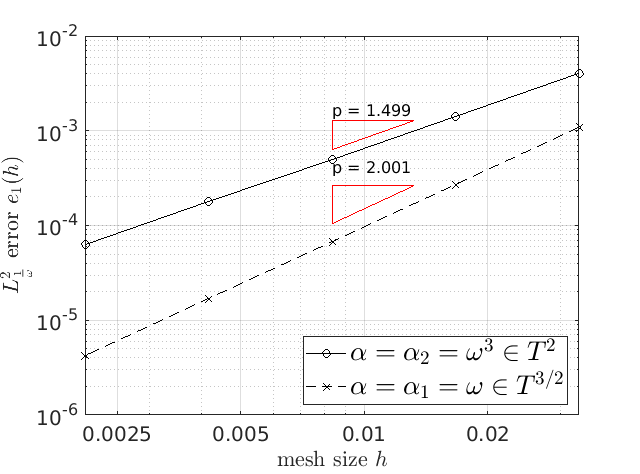
\includegraphics[scale = 0.4]{figs/ordreCVDir}
	\caption{Effective order of convergence of the approximation of the solution $\alpha$ to \eqref{Somegaalpha} by the weighted Galerkin method. The blue data correspond to a case where $\alpha \in T^{s}$ for all $s < \frac{3}{2}$ but $\alpha \notin T^{3/2}$. In this case, the theory predicts a $O(h^{3/2})$ rate of convergence, which is what we observe in practice. The red data corresponds to a case where $\alpha \in T^s$. In this case, a $O(h^2)$ rate of convergence is predicted by the theory and indeed observed here.} 
	\label{fig:errL2dir}
\end{figure}
\begin{figure}
	\centering
	\hspace{-1cm}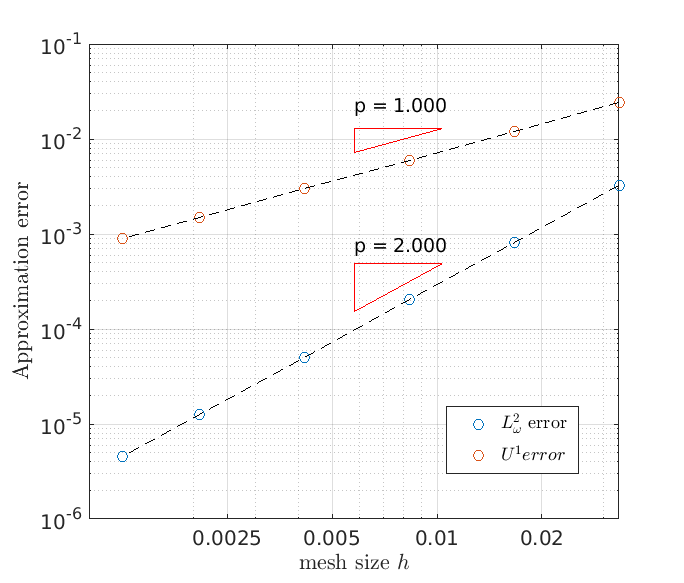
\includegraphics[scale = 0.4]{figs/ordreCVNeu}
	\caption{Effective order of convergence of the approximation of the solution $\beta$ to \eqref{Nomegabeta} by the weighted Galerkin method. The second member is taken as $u_N = U_2 \in U^{\infty}$, and the solution is therefore $\beta = \frac{2}{3}U_2$. We plot in blue the $L^2_\omega$ error $\norm{\beta - \beta_h}_{\omega}$ and in red the $U^1$ error $\norm{\beta - \beta_h}_{U^1}$. Here the theory predicts the $O(h)$ order of convergence for the second curve. The $O(h^2)$ order of the first curve is not yet explained by our theory.} 
	\label{fig:errL2Neu}
\end{figure}


%\subsection{Numerical quadratures and compression method}
%\paragraph{Weakly singular kernels.} 
%\todo{Je serais d'avis de supprimer cette section et de citer EBD plus tard}
%To compute the elements of the matrix of the operators with weakly singular kernel, we use Gaussian quadratures 
%for the weights $\frac{1}{\omega}$ and $\omega$, with $3$ points on each segment. As a result, we obtain a vector $(x_k)_k$ of $3N$ points in $\R^2$ 
%and a vector $(w_k)$ of $3N$ quadrature weights. If $p$ stands for the weight ($1/\omega$ or $\omega$), then quantities of the form 
%$\int_\Gamma \int_\Gamma  p(x)p(y)\phi_i(x) G_k(x,y) \phi_j(y)$, are approximated by
%\begin{equation}
%\label{approxDoubleIntegral}
%\int_\Gamma \int_\Gamma   p(x)p(y)\phi_i(x) G_k(x,y) \phi_j(y) \approx \sum_{k = 1}^N w_k \phi_i(x_k) \sum_{l = 1}^N  w_l G(x_k,x_l) \phi_j(x_l).
%\end{equation}
%Since the kernel $G_k$ is singular, we must correct the previous formula when $x_k$ and $x_l$ are close from each other. This is done by the following 
%method. For each segment $I_n$ in the mesh, we find the subset $(x_k')$of the points $x_k$ that are closer than a fixed threshold from $I_n$. For those 
%points, we compute more accurately the integral 
%\[ \int_{I_n} p(y)G_k(x_k,y) \phi_j(y),\]
%by any method at our disposal (change of variable, subtraction of the singularity among others, see for instance \cite{sauter2011boundary}). The second 
%integral is then approximated using the previous quadrature. 
%Note that in this framework, the addition of the weight $p$ only requires minor modification over a standard BEM code. Basically, one only needs to 
%compute numerical quadratures for the weight $p$, for which open source routines are available, and implement a method to compute the close integrals 
%with the weight $p$. Using the variable change $x = \cos(\theta)$, the weight disappears and the only singularity left is that of $G_k$. 
%
%\paragraph{Hypersingular operator.} Although the weighted hypersingular $N_{k,\omega}$ operator has a non-integrable kernel, we have the formula
%\[\duality{N_{k,\omega} \beta}{\beta'}_\omega = \duality{S_{k,\omega}\left(\omega \partial_x \omega \right)u}
%{\left(\omega \partial_x \omega \right) v}_\frac{1}{\omega} - k^2 \duality{S_\omega \omega^2 u}{\omega^2 v}_\frac{1}{\omega}.\]
%This only involves weakly singular kernels and is thus treated by the previous method. 
%
%\paragraph{Compression method} The rhs of \eqref{approxDoubleIntegral} is the scalar product of a vector with a discrete convolution. To accelerate 
%the computation and to avoid assembling the full matrix $(G_k(x_k,x_l))$, we use \toDo{Citer EBD alors que pas encore accepté ?}. 
%
\subsection{Preconditioning the linear systems}
Let $X_h$ the considered finite element space ($X_h = V_h$ or $W_h$), and $(\phi_i)_{i}$ the basis functions. For an operator $A$, we denote by $\left[A\right]_p$ 
the Galerkin matrix of the operator \toDo{for the relevant weight $p(x) = \frac{1}{\omega(x)}$ or $\omega(x)$}, defined by
$$
[A]_{p,ij} = \int_\Gamma (A\phi_j)(x) \phi_i(x) p(x)\,dx\,.
$$
When the operator $BA$ is a compact perturbation of the identity (either in $T^s$ or $U^s$) then, following \cite{steinbach1998construction}, we 
precondition the linear system $\left[A\right]_p x = b$ by the matrix $\left[I_d\right]^{-1}_p \left[B\right]_p \left[I_d\right]_p^{-1}$, which amounts to solve
$$
\left[I_d\right]^{-1}_p \left[B\right]_p \left[I_d\right]_p^{-1} [A]_p x = \left[I_d\right]^{-1}_p \left[B\right]_p \left[I_d\right]_p^{-1} b\,.
$$
When $B$ is the inverse of a local operator $C$, then it may be more convenient to compute $\left[C\right]_p$, and solve instead
$$
\left[C\right]_p^{-1}[A]_p x = \left[C\right]_p^{-1}b\,.
$$
%When testing the pair $S_{k,\omega}, N_{k,\omega}$ as mutual preconditioner, the 
%operator $S_{k,\omega}N_{k,\omega}$ is discretized as $\left[I_d\right]_\frac{1}{\omega}^{-1} \left[S_{k,\omega}\right]_\frac{1}{\omega}\left[I_d\right]_{\omega}^{-1}\left[N_{k,\omega}\right]_\omega$, yielding very satisfactory results. 

The preconditioners introduced in this work are in the form of square roots of local operators. More precisely, we introduced two preconditioners $P_1$ and $P_2$ with 
\begin{eqnarray*}
	P_1(k) &=& \left(-(\omega \partial_x)^2 - k^2 \omega^2\right)^{1/2}\\
	P_2(k) &=& \left(-(\partial_x \omega)^2 - k^2 \omega^2 \right)^{-1/2}
\end{eqnarray*}
For the second equation, we rewrite 
\[P_2(k) = \left(-(\partial_x \omega)^2 - k^2 \omega^2 \right)^{-1} \left(-(\partial_x \omega)^2 - k^2 \omega^2 \right)^{1/2},\]
which brings us back to computing the square root of a sparse matrix. When the frequency is $0$, we use the method exposed in \cite{hale2008computing}. 
When the frequency is non-zero, the previous method fails since the spectrum of the matrix contains negative values. In \cite{antoine2007generalized}, a 
method involving a Pad\'e approximation of the square root, with a rotated branch cut, is used to compute the matrix of an operator of the form 
$\sqrt{X - k^2 I_d}$ where $X$ is a positive definite operator. This method gives excellent results in our context when using 
$X = -(\partial \omega_x)^2 + k^2 \left(I_d - \omega^2\right)$. Specifically, we build a rational approximation of the function $X \mapsto \sqrt{X - k^2}$ in the form
\[\sqrt{X - k^2} = a_0 + \sum_{i = 0}^{N_p} \frac{a_i}{b_i + X}\,.\]
We then take
\[\left[\sqrt{X - k^2 I_d}\right]_p \approx a_0[I_d]_p + \sum_{i = 0}^{N_p} a_i\left(b_i[I_d]_p + [X]_p\right)^{-1}\,.\]

%%%%%%%%%%%%%%%%%%%%%%%%%%%%%%%%%%%%
\subsection{Numerical results}
\label{sec:NumericalResutls}

All the numerical results exposed here are obtained on a personal laptop running on an eight cores intel i7 processor with a clock rate of 2.8GHz. 
The Galerkin method has been implemented in the language Matlab R2018. 


\paragraph{Flat segment, Laplace-Dirichlet problem.} 
In \autoref{TableNitTimeLaplaceDirichlet}, we report the number of iterations for the numerical resolution of the Laplace problem \eqref{Somegaalpha} 
by the method detailed above, in \autoref{sec:numerMeth}. Two cases are considered, first without any preconditioner, and then with a preconditioner given 
by $[I_d]_\frac{1}{\omega}^{-1} \left[B \right]_\frac{1}{\omega} [I_d]_\frac{1}{\omega}^{-1}$ where
$[B]_\frac{1}{\omega}$ is the Galerkin matrix of the operator $\sqrt{ -(\omega \partial_x)^2 + \frac{1}{\ln(2)^2} \pi_0}$. The right hand 
side in \eqref{Somegaalpha} is chosen as $u_D(x) = (x^2 + 0.001)^{-1/2}, x \in [-1,1]$. A graph of the residual along the iterations is given in \autoref{FigureNitLaplaceDirichlet} for a graded mesh with 1600 node points. 

\begin{table}[H]
	\begin{center}
		\begin{tabular}{m{4em}|m{4em}|m{4em}|m{4em}| m{4em}} 
			\hline
			\multicolumn{1}{c|}{ }&
			\multicolumn{2}{c|}{with Prec.}&\multicolumn{2}{c}{without Prec.}\\
			\hline
			$N$ & $n_{it}$& t(s) & $n_{it}$ & t(s)\\
			\hline\hline
			50 & 7 & 0.11 & 35 & 0.21\\
			\hline
			200 & 7 & 0.14 & 53 & 0.55\\
			\hline
			800 & 7 & 0.29 & 76 & 2.0 \\
			\hline
			3200 & 7 & 0.95 & 107 & 9.5\\
			\hline
		\end{tabular}
		\caption{Number of iteration and time needed for the numerical resolution of \eqref{Somegaalpha} using Galerkin finite elements with and without preconditioner.}
		\label{TableNitTimeLaplaceDirichlet}
	\end{center}
\end{table}
\begin{figure}[H]
	\centering
	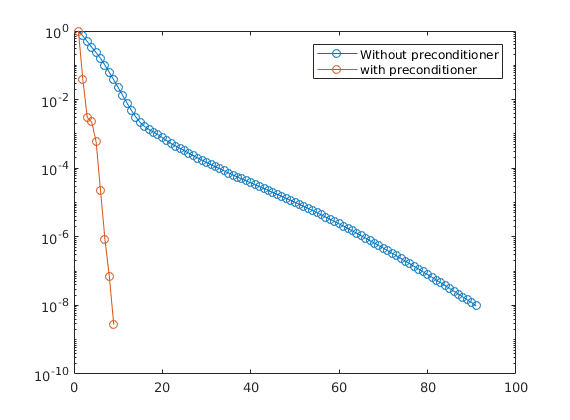
\includegraphics[scale=0.7]{figs/PrecondDirichletLaplaceSeg.png}
	\caption{Number of iteration in the resolution of the single layer integral equation with a mesh of size $N = 1600$.}
	\label{FigureNitLaplaceDirichlet}
\end{figure}

\paragraph{Flat segment, Laplace-Neumann problem.} 
For the Neumann problem \eqref{Nomegabeta}, we also report in \autoref{TableNitTimeLaplaceNeumann} the number of iterations for the 
numerical resolution with and without the preconditioner given by $[I_p]^{-1}_{\omega} \left[C \right]_\omega [I_p]^{-1}_{\omega}$ where $\left[ C \right]_\omega$ 
is the Galerkin matrix of the operator $\sqrt{ -( \partial_x \omega)^{-2}}$. The right hand side in \eqref{Nomegabeta} is chosen as 
$u_N(x) = (x^2 + 0.001)^{1/2}, x \in [-1,1]$. The decay of the residual along the iterations is shown in Fig. \ref{FigureNitLaplaceNeumann}.

\begin{table}[H]
	\begin{center}
		\begin{tabular}{m{4em} | m{4em} | m{4em} | m{4em} | m{4em}} 
			\hline
			\multicolumn{1}{c|}{ }&
			\multicolumn{2}{c|}{with Prec.}&\multicolumn{2}{c}{without Prec.}\\
			\hline
			$N$ & $n_{it}$& t(s) & $n_{it}$ & t(s)\\
			\hline\hline
			50 & 4 & 0.09 & 50 & 0.31\\
			\hline
			200 & 4 & 0.12 & 200 & 2.0\\
			\hline
			800 & 4 & 0.56 & 799 & 30 \\
			\hline
			3200 & 4 & 17.7 & 3007 & 630\\
			\hline
		\end{tabular}
	\end{center}
	\caption{Number of iteration and time needed for the numerical resolution of \eqref{Somegaalpha} using Galerkin finite elements with and without preconditioner.}
	\label{TableNitTimeLaplaceNeumann}
\end{table}
\vspace{-0.7cm}
\begin{figure}[H]
	\centering
	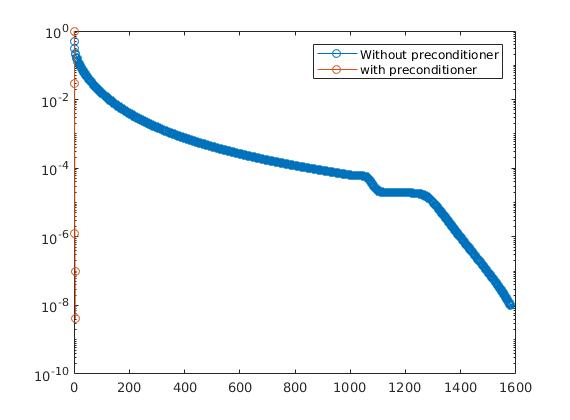
\includegraphics[scale=0.5]{figs/PrecondNeumannLaplaceSeg.png}
	\caption{Number of iteration in the resolution of the hypersingular  integral equation with a mesh of size $N = 1600$. The importance of preconditioning 
	in this case is even more spectacular than in the case of the single-layer equation.}
	\label{FigureNitLaplaceNeumann}
\end{figure}
We observe in both Dirichlet and Neumann cases a drastic decay of the number of iteration which justifies the approach. We also see that, 
as expected, the number of iterations obtained with the preconditioned version does not depend on the mesh.

\vspace*{0.5cm}

We now turn our attention to Helmholtz equation. In each case, in order to fully resolve the frequency, the number of segments in the 
discretization is set to $N \approx 10k$, where $k = \frac{\pi}{\lambda}$ is the wavenumber. In the GMRES iteration, we require a relative 
residual below $10^{-8}$. 

\paragraph{Flat segment, Helmholtz-Dirichlet problem.} 
In \autoref{TableNitTimeHemholtzDirichlet} we report the number of GMRES iterations for the numerical resolution of Equation \eqref{Sklambda} 
on the segment $\Gamma = [-1,1]\times \{0\}$, when the linear system is preconditioned by the operator $\sqrt{-(\omega \partial_x)^2 - k^2 \omega^2}$, as 
compared to the case where no preconditioner is used.  We take, for the Dirichlet data, the plane wave $u_D(x) = e^{ikx}$. We also provide, in 
\autoref{FigureNitHelmDirichlet}, the value of the relative residual in the GMRES method along the iterations, with and without preconditioner, 
for a problem with $L = 800 \lambda$. As before, we see that the number of iterations needed to reach a given precision decreases significantly but, this time, 
we observe a very slight increase with respect to the wavenumber. 
\todo{en maillage à fréquence fixée, c'est bien indépentdant donc j'ai remplacé with respect to "mesh size" par "wavenumber"}
\begin{table}[H]
	\begin{center}
		\begin{tabular}{m{4em} | m{4em} | m{4em} | m{4em} | m{4em}} 
			\hline
			\multicolumn{1}{c|}{ }&
			\multicolumn{2}{c|}{with Prec.}&\multicolumn{2}{c}{without Prec.}\\
			\hline
			$L/\lambda$ & $n_{it}$& t(s) & $n_{it}$ & t(s)\\
			\hline\hline
			50 & 8 & 0.1 & 73 & 0.28\\
			\hline
			200 & 10 & 1.3 & 116 & 17\\
			\hline
			800 & 15 & 34 & 148 & 300\\
			\hline
		\end{tabular}
	\end{center}
	\caption{Number of iterations and time needed for the numerical resolution of \eqref{Somegaalpha} using Galerkin finite elements with and without preconditioner.}
	\label{TableNitTimeHemholtzDirichlet}
\end{table}
\vspace{-1cm}
\begin{figure}[H]
	\centering
	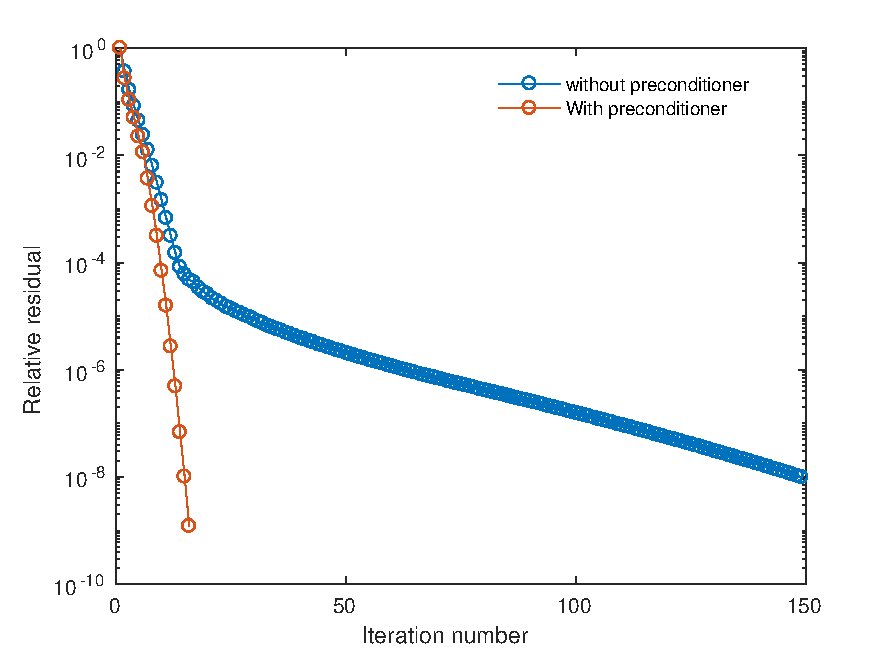
\includegraphics[scale=0.5]{figs/PrecondDirichletHelmSegPDF}
	\caption{Number of iteration in the resolution of the single layer integral equation with a mesh of size $N \approx 3700$, $L = 800 \lambda$.}
	\label{FigureNitHelmDirichlet}
\end{figure}

\paragraph{Flat segment, Helmholtz-Neumann problem.} 
Finally, to end up this validation stage, we run the same numerical comparisons, this time solving \eqref{Nkmu} and considering the preconditioning operator 
$\left(-(\partial_x \omega)^2 - k^2 \omega^2\right)^{-1/2}$. Results are given in \autoref{TableNitTimeHemholtzNeumann} for different meshes and in
\autoref{FigureNitHelmNeumann} for the evolution of the residual along the iterations. Huge differences, btoh in time and number of iterations are
shown in favor of the preconditioned system.
\begin{table}[H]
	\begin{center}
		\begin{tabular}{m{4em} | m{4em} | m{4em} | m{4em} | m{4em}} 
			\hline
			\multicolumn{1}{c|}{ }&
			\multicolumn{2}{c|}{with Prec.}&\multicolumn{2}{c}{without Prec.}\\
			\hline
			$L/\lambda$ & $n_{it}$& t(s) & $n_{it}$ & t(s)\\
			\hline\hline
			50 & 8 & 0.08 & 785 & 9.4\\
			\hline
			200 & 10 & 3.6 & $> 2000$ &  $>$ 2min\\
			\hline
			800 & 17 & 73 & $>2000$ &  $>$ 2min\\
			\hline
		\end{tabular}
	\end{center}	
	\caption{Number of iteration and time needed for the numerical resolution of \eqref{Somegaalpha} using Galerkin finite elements with and without preconditioner.}
	\label{TableNitTimeHemholtzNeumann}
\end{table}
\vspace{-1cm}
\begin{figure}[H]
	\centering
	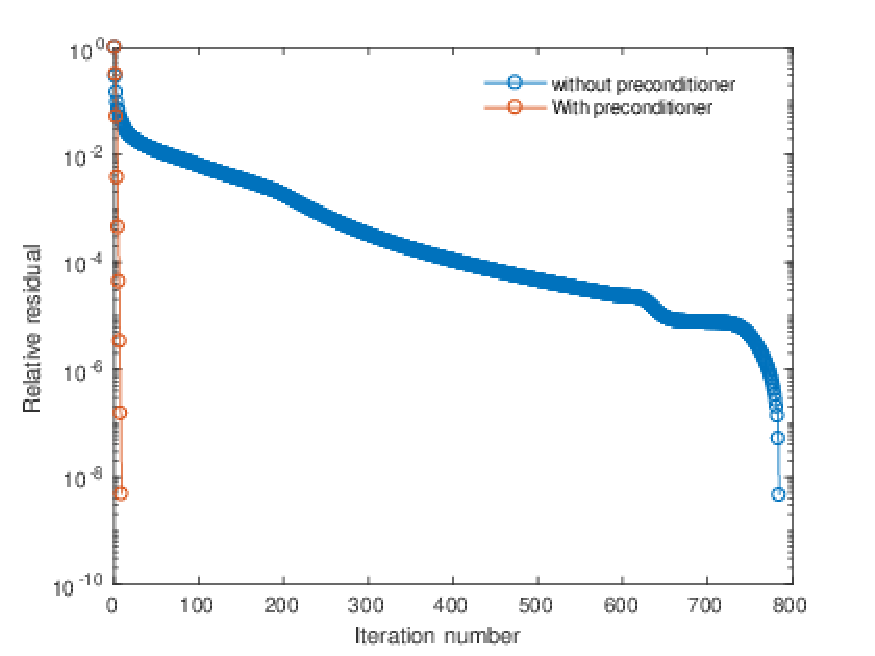
\includegraphics[scale=0.5]{figs/PrecondNeumannHelmSegPDF}
	\caption{Number of iteration in the resolution of Hypersingular integral equation with a mesh of size $N \approx 800$, $L = 50 \lambda$.}
	\label{FigureNitHelmNeumann}
\end{figure}

\paragraph{Non-flat arc.} Here, we also report numerical results when the curve is a portion of spiral (see \autoref{ArcOfSpiral}), for both boundary conditions. This shows that the preconditioning strategy is also efficient in presence of non-zero curvature. 
\begin{table}[H]
	\begin{center}
		\begin{tabular}{m{4em} | m{4em} | m{4em} | m{4em} | m{4em}} 
			\hline
			\multicolumn{1}{c|}{ }&
			\multicolumn{2}{c|}{With prec.}&\multicolumn{2}{c}{Without prec.}\\
			\hline
			$L/\lambda$ & $n_{it}$& t(s) & $n_{it}$ & t(s)\\
			\hline\hline
			50 & 23 & 0.6 & 785 & 9.4\\
			\hline
			200 & 27 & 9 & $> 2000$ &  $>$ 2min\\
			\hline
			800 & 40 & 35& $> 2000$ &  $>$ 2min\\
			\hline
		\end{tabular}
	\end{center}
	\caption{Computing times and number of iterations for the spiral-shaped arc.}
\end{table}
\vspace{-1cm}
\begin{figure}[H]
	\centering
	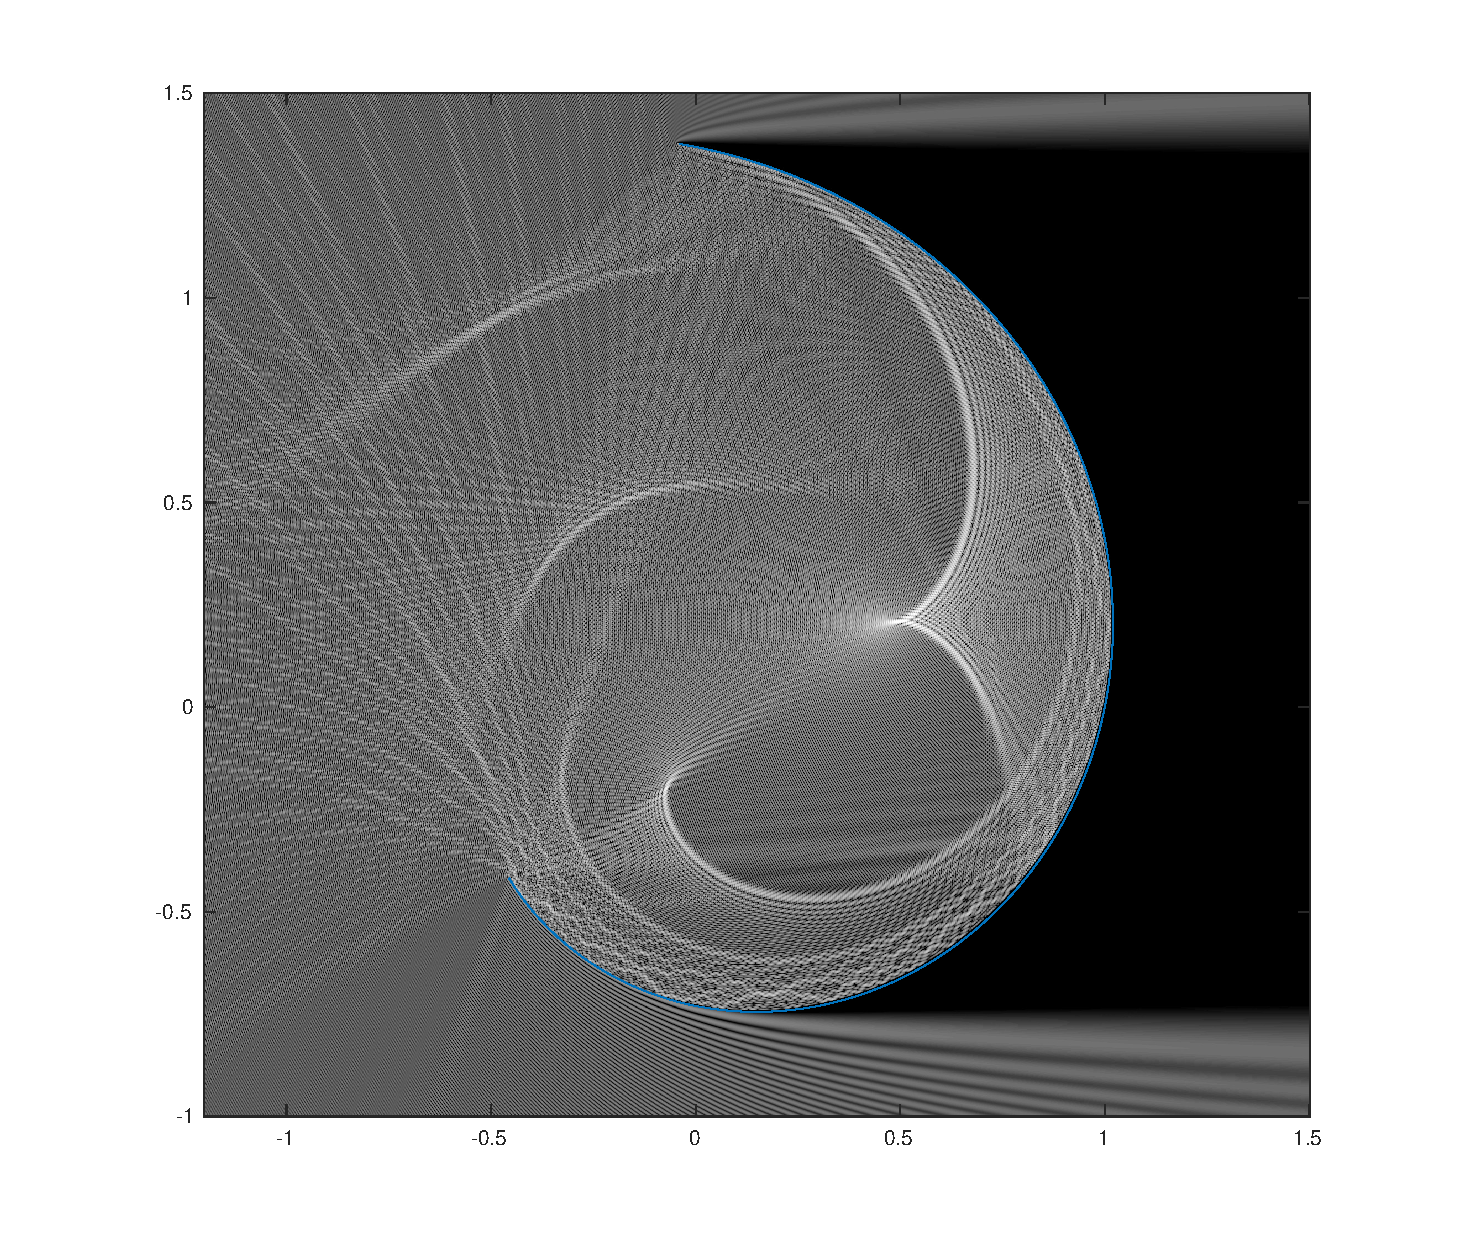
\includegraphics[width=\linewidth]{figs/arcOfSpiral800_3}
	\vspace{-1.2cm}
	\caption{Sample diffraction pattern (Dirichlet boundary conditions) with left to right incidence for an arc of spiral of size $L = 800 \lambda$. 
	After the resolution of the integral equation, the computation of the image is accelerated by the EBD method \cite{averseng2017}.}
	\label{ArcOfSpiral}
\end{figure}

\paragraph{Comparison with the generalized Calderon relations.} Eventually, we test the idea that was presented in \cite{bruno2012second}, namely 
to use $S_{k,\omega}$ and $N_{k,\omega}$ as mutual preconditioners. This alternative method is also very efficient in our numerical setting (here, we use 
simple piecewise affine functions, whereas in \cite{bruno2012second}, spectral discretization with trigonometric polynomials is used). We report in 
\autoref{TableBrunoVsSqrt} the number of iterations and computing times for the Neumann problem with an angle of incidence $\frac{\pi}{4}$ on the 
flat segment. The number of iterations is comparable for both methods. However, the matrix-vector product time in our method is significantly 
slower as it only involves sparse operators. This leads to a faster resolution of the linear system. 

\begin{table}[H]
	\begin{center}
		\begin{tabular}{m{4em} | m{4em} | m{4em} | m{4em} | m{4em}} 
			\hline
			\multicolumn{1}{c|}{ }&
			\multicolumn{2}{c|}{Calderon Prec.}&\multicolumn{2}{c}{Square root Prec.}\\
			\hline
			$L/\lambda$ & $n_{it}$& t(s) & $n_{it}$ & t(s)\\
			\hline\hline
			50 & 14 & 0.1 & 8 & 0.1\\
			\hline
			200 & 15 & 7.5 & 11 &  3.6\\
			\hline
			800 & 16 & 130 & 15 & 70\\
			\hline
		\end{tabular}
	\end{center}
	\caption{Number of iteration and time needed for the numerical resolution of \eqref{Sklambda} using Galerkin finite elements with and without preconditioner.}
	\label{TableBrunoVsSqrt}
\end{table}
	
%%%%%%%%%%%%%%%%%%%%%%%%%%%
\section{Conclusion} 
We have presented a new approach for the preconditioning of integral equations coming from the discretization of wave scattering problems
in 2D by open arc domains. The methodology is very effective and proven to be optimal for Laplace problems on straight segments. It has
three advantages:
\begin{itemize}
\item It generalizes the formulas mainly proposed in \cite{antoine2007generalized} for regular domains, which is only modified by a suitable weight.
\item We can show that one can recover optimal error estimates, provided that the mesh is suitably graded near the edges.
\item Eventually, a novel pseudo-differential approach, adapted to the corner singularities that appear in the problem is proposed.
It is sketched in the present paper, but given in full details in \cite{averseng}.
\end{itemize}
We deeply believe that the methodology opens new perspectives for such problems. First, a generalization to specific 3D scattering
problem, e.g. by a flat disc seems a simple generalization. We plan to extend the results presented here to such problems in the very
near future. Second, the strategy that we used here seems very likely to be extended to the half line and hopefully to 2D sectors, giving,
on the one hand a new pseudo-differential analysis more suitable than classical ones (see e.g. \cite{melrose,olapaivarinta,schulze1,schulze2})
for handling Helmholtz-like problems on singular domains, and, on the other hand, a completely new preconditioning  technique adapted
to the treatment of BEM operators on domains with corners or wedges in 3D. Eventually, the weighted square root operators that appeared
in the present context might well be generalized to give suitable approximation of the exterior Dirichlet to Neumann map for the Helmholtz equation
which is of particular importance in e.g. domain decomposition methods. Having such approximations might therefore lead to better
methods in that context too.
	
%\appendix
%\section{Commutation of $N_\omega$ and $(\partial_x \omega)^2 + k^2\omega^2$}
%\label{ann:commut}
%\begin{Lem}
%	\label{dxSomega2=Somegadxomega}
%	For any $\phi$, there holds 
%	\[\partial_x S_\omega \omega^2 \phi = S_\omega \omega \partial_x \omega \phi.\]
%\end{Lem}
%\begin{proof}
%	In our context, the largest space encountered is $U^{- \infty}$ (As a consequence of \autoref{inclusionsTsUs}) so we shall show that this identity holds in that space.
%	For any $s$, $\omega^2$ is a continuous operator from $U^s$ to $T^s$, $S_\omega$ is continuous from $T^s$ to $T^{s+1}$ and $\partial_x$ is continuous from $T^{s+1}$ to $U^s$. Indeed, we have 
%	\[\omega^2 U_n = \frac{T_n - T_{n+2}}{2}\] 
%	and 
%	\[\partial_x T_n = n U_{n-1}.\]
%	Therefore, the left operator is continuous from $U^s$ to $U^s$. Similarly, the right operator is continuous from $U^{s}$ to $U^s$ for all $s$. If we fix $\phi \in U^{s}$ for some $s$, using the decomposition of $\phi$ on $U_n$, there exists a sequence $\phi_N$ in $U^{\infty}$ converging to $\phi$ in $U^{s}$. It is thus sufficient to check the identity for $\phi = U_n$. For $n \geq 1$, 
%	\begin{eqnarray*}
%		\partial_x S_\omega \omega^2 U_n &=& \partial_x S_\omega \left(\frac{T_{n} - T_{n+2}}{2}\right)\\
%		&=& \partial_x\left(\frac{T_{n}}{4n} - \frac{T_{n+2}}{4(n+2)} \right)\\
%		&=& \frac{U_{n-1} - U_{n+1}}{4}\\
%		&=& -\frac{T_{n+1}}{2}.
%	\end{eqnarray*}
%	One can check that the result also holds for $n = 0$. On the other hand, for all $n$, 
%	\begin{eqnarray*}
%		S_\omega \omega \partial_x \omega U_n &=&-(n+1) S_\omega T_{n+1}\\
%		&=& -\frac{1}{2}T_{n+1}
%	\end{eqnarray*}
%	which proves the result. 
%\end{proof}
%We now turn to the proof of the theorem. To ease the computations, we take some notations: let $\Delta_\omega \isdef (\omega \partial_x)^2$, $\Delta_\omega^T \isdef (\partial_x \omega)^2$,  $N_\omega \isdef N_{k,\omega}$, and $S_\omega \isdef S_{k,\omega}$. Using, equation \eqref{NkenfonctiondeSk} we can write 
%\[N_\omega = -\partial_x S_\omega \omega \partial_x \omega - k^2 S_\omega \omega^2.\]
%To show that $N_\omega$ and $\Delta_\omega^T + k^2\omega^2$ commute, we compute their commutator $C$ and show that it is null. 
%We have 
%\begin{eqnarray*}
%	C &\isdef& N_\omega \Delta_\omega^T - \Delta_\omega^T N_\omega + k^2N_\omega \omega^2 - k^2 \omega^2 N_\omega \\
%	&=& -\partial_x S_\omega \Delta_\omega \omega \partial_x \omega  - k^2 S_\omega \omega^2 \Delta_\omega^T \\
%	&& + \partial_x \Delta_\omega S_\omega \omega \partial_x \omega + k^2 \Delta_\omega^T S_\omega \omega^2 \\
%	&& - k^2 \partial_x S_\omega \omega \partial_x \omega^3 - k^4 S_\omega \omega^4 \\
%	&& + k^2 \omega^2 \partial_x S_\omega \omega \partial_x \omega + k^4 \omega^2 S_\omega \omega^2
%\end{eqnarray*}
%where each term in the r.h.s. of the first equality gives rise to a line in the second. We rearrange the terms as follows:
%\begin{eqnarray*}
%	C &=& \partial_x (\Delta_\omega S_\omega - S_\omega \Delta_\omega) \omega \partial_x \omega - k^2 \partial_x S_\omega \omega \partial_x \omega^3 + k^2 \omega^2 \partial_x S_\omega \omega\partial_x \omega\\	
%	&& + k^4 (\omega^2 S_\omega - S_\omega \omega^2) \omega^2\\
%	&& + k^2(\Delta_\omega^T S_\omega \omega^2 - S_\omega \omega^2 \Delta_\omega^T)
%\end{eqnarray*}
%For the first term, we inject the commutation shown in \autoref{commutations}. For the last line, we use the following identities: 
%\[ \Delta_\omega^T = \Delta_\omega - 2x \partial_x - 1\]
%\[ \omega^2 \Delta_\omega^T = \Delta_\omega \omega^2 + \omega^2 + 2 \omega x \partial_x \omega\]
%Let $D = \frac{C}{k^2}$, 
%\begin{eqnarray*}
%	D &=& \partial_x S_\omega \omega (\omega^2\partial_x - \partial_x \omega^2) \omega  + (\omega^2 \partial_x - \partial_x \omega^2)S_\omega \omega \partial_x \omega\\
%	&&+ k^2(\omega^2 S_\omega - S_\omega \omega^2) \omega^2\\
%	&&+ (\Delta_\omega - 2x \partial_x - 1)S_\omega \omega^2 - S_\omega(\Delta_\omega \omega^2 + \omega^2 + 2\omega x \partial_x \omega) 
%\end{eqnarray*}
%We use $\omega^2 \partial_x - \partial_x \omega^2 = 2x$, and the relation $\partial_x S \omega^2 = S_\omega \omega \partial_x \omega$ to get
%\begin{eqnarray*}
%	D &=& 2 S_\omega \omega \partial_x x\omega + 2 x S_\omega  \omega \partial_x \omega \\
%	&& + \left(k^2(\omega^2 S_\omega - S_\omega \omega^2) + \Delta_\omega S_\omega - S_\omega \Delta_\omega \right)\omega^2\\
%	&& - 2 S_\omega \omega^2 - 2 x  S_\omega \omega \partial_x \omega - 2 S_\omega \omega x \partial_x \omega.
%\end{eqnarray*}
%Using again the commutation shown in \autoref{commutations}, we are left with 
%\begin{eqnarray*}
%	D &=&  2 S_\omega \omega (\partial_x x - x \partial_x) \omega - 2 S_\omega \omega^2
%\end{eqnarray*}
%This is null since $\partial_x x - x \partial_x = 1$. 

\begin{thebibliography}{10}

\bibitem{alouges2015sparse}F. Alouges and M. Aussal. \newblock The Sparse Cardinal Sine Decomposition and its application for fast numerical convolution. \newblock{\em Numerical Algorithms}, 70(2), 2015.

\bibitem{alouges2013simple}F. Alouges, J. Bourguignon-Mirebeau and D. Levadoux. 
\newblock A simple preconditioned domain decomposition method for electromagnetic scattering problems. \newblock {\em J. Comput. Math.}, 31(1), 2013.

\bibitem{alouges2007stable}F. Alouges, S. Borel and D. Levadoux. 
\newblock A Stable well conditioned integral equation for electromagnetism scattering, \newblock{\em J. Comput. Appl. Math.} 204(2):440--451, 2007.

\bibitem{alouges2005new}F. Alouges, S. Borel and D. Levadoux.
\newblock  A new well-conditioned integral formulation for Maxwell equations in three-dimensions. 
\newblock{\em IEEE Trans. on Antennas and Propagation} 53(9), 2005.

\bibitem{antoine2007generalized}
X. Antoine and M. Darbas.
\newblock Generalized combined field integral equations for the iterative
  solution of the three-dimensional helmholtz equation.
\newblock {\em ESAIM: Mathematical Modelling and Numerical Analysis},
  41(1):147--167, 2007.

\bibitem{atkinson1991numerical}
K.~E. Atkinson and I.~H. Sloan.
\newblock The numerical solution of first-kind logarithmic-kernel integral
  equations on smooth open arcs.
\newblock {\em mathematics of computation}, 56(193):119--139, 1991.

\bibitem{averseng}M. Averseng,
\newblock New preconditioners for Laplace and  Helmholtz integral equation on open curves: II. Theoretical analysis.
\newblock {\em Submitted}.

\bibitem{averseng2017}
M. Averseng. 
\newblock Fast discrete convolution in $\mathbb{R}^2$ using sparse Bessel Decomposition.
\newblock accepted for publication in {\em Numerical Algorithms}, 2018 and {\em arXiv:1711.07877 [math.NA]}, 2017.

\bibitem{betcke2014spectral}
T.~Betcke, J.~Phillips, and E. A.~Spence.
\newblock Spectral decompositions and nonnormality of boundary integral
  operators in acoustic scattering.
\newblock {\em IMA Journal of Numerical Analysis}, 34(2):700--731, 2014.

\bibitem{bruno2012second}
O.~P. Bruno and S.~K. Lintner.
\newblock Second-kind integral solvers for te and tm problems of diffraction by
  open arcs.
\newblock {\em Radio Science}, 47(6), 2012.

\bibitem{christiansen2002preconditioner}
S.~H. Christiansen and J.-C. N{\'e}d{\'e}lec.
\newblock A preconditioner for the electric field integral equation based on
  calderon formulas.
\newblock {\em SIAM Journal on Numerical Analysis}, 40(3):1100--1135, 2002.

\bibitem{costabel1988convergence}
M. Costabel, V.~J. Ervin, and E.~P. Stephan.
\newblock On the convergence of collocation methods for Symm's integral
  equation on open curves.
\newblock {\em Mathematics of computation}, 51(183):167--179, 1988.

\bibitem{Darbas2005}
M.~Darbas.
\newblock Generalized combined field integral equations for the iterative
  solution of the three-dimensional maxwell equations.
\newblock {\em Applied Mathematics Letters}, 19(8):834--839, 2006.

\bibitem{hale2008computing}
N. Hale, N.~J. Higham, and L.~N. Trefethen.
\newblock Computing a\^{}$\alpha$,$\backslash$log(a), and related matrix
  functions by contour integrals.
\newblock {\em SIAM Journal on Numerical Analysis}, 46(5):2505--2523, 2008.

\bibitem{hiptmair2014mesh}
R. Hiptmair, C. Jerez-Hanckes, and C. Urzua-Torres.
\newblock Mesh-independent operator preconditioning for boundary elements on
  open curves.
\newblock {\em SIAM Journal on Numerical Analysis}, 52(5):2295--2314, 2014.

\bibitem{hiptmair2017closed}
R. Hiptmair, C. Jerez-Hanckes, and C. Urzua-Torres.
\newblock Closed-form exact inverses of the weakly singular and hypersingular
  operators on disks.
\newblock {\em arXiv preprint arXiv:1703.08556}, 2017.

\bibitem{jerez2012explicit}
C. Jerez-Hanckes and J.-C. N{\'e}d{\'e}lec.
\newblock Explicit variational forms for the inverses of integral logarithmic
  operators over an interval.
\newblock {\em SIAM Journal on Mathematical Analysis}, 44(4):2666--2694, 2012.

\bibitem{jiang2004second}
S. Jiang and V. Rokhlin.
\newblock Second kind integral equations for the classical potential theory on
  open surfaces ii.
\newblock {\em Journal of Computational Physics}, 195(1):1--16, 2004.

\bibitem{LevadouxM2AS07}
{D. P.} Levadoux.
\newblock Some preconditioners for the {CFIE} equation of electromagnetism.
\newblock {\em Math. Meth. Appl. Sci.}, 17:2015--2028, 2008.

\bibitem{LevadouxMillotPernet}
{D. P.} Levadoux, {F.} Millot, and {S.} Pernet.
\newblock New trends in the preconditioning of integral equations of electromagnetism.
\newblock {\em Springer-Verlag Berlin Heifelberg}, Scientific Computing in Electrical Engineering SCEE 2008 by Janne Roos, Luis R. J. Costa
(Mathematics in industry 14) 383--394, 2010.

\bibitem{mason2002chebyshev}
J.~C. Mason and D.~C. Handscomb.
\newblock {\em Chebyshev polynomials}.
\newblock CRC Press, 2002.

\bibitem{mclean2000strongly}
W. C.~H. McLean.
\newblock {\em Strongly elliptic systems and boundary integral equations}.
\newblock Cambridge university press, 2000.

\bibitem{LeanTran97}
{W. C. H. McLean, T. Tran}.
\newblock A preconditioning strategy for boundary element galerkin methods.
\newblock {\em Numer. Methods for Partial Differential Equations}, 13:283--301 1997.

\bibitem{melrose} R. Melrose. Transformation of boundary problems. \newblock{\em Acta Mathematica}. 147:149--236, 1981.


\bibitem{monch1996numerical}
Lars M{\"o}nch.
\newblock On the numerical solution of the direct scattering problem for an
  open sound-hard arc.
\newblock {\em Journal of computational and applied mathematics},
  71(2):343--356, 1996.

\bibitem{Nedelec01}
J.-C. Nedelec. \newblock {\em Acoustic and Electromagnetic Equations, integral representations
  for harmonic problems}. \newblock Springer, 2001.

\bibitem{NIST:DLMF}
F.~W.~J. Olver, A.~B. Olde~Daalhuis, D.~W. Lozier, B.~I. Schneider, R.~F.
  Boisvert, C.~W. Clark, B.~R. Miller, and B.~V. Saunders.
\newblock {\it NIST Digital Library of Mathematical Functions}.
\newblock http://dlmf.nist.gov/, Release 1.0.16 of 2017-09-18.

\bibitem{olapaivarinta} P. Ola and L. P\"aiv\"arinta, {\em Mellin operators and pseudodifferential operators on graphs}, Waves Random Media {\bf 14} (2004) S129-S142.

\bibitem{postell1990h}
F. V.~Postell and E.~P. Stephan.
\newblock On the h-, p-and hp versions of the boundary element
  method?numerical results.
\newblock {\em Computer Methods in Applied Mechanics and Engineering},
  83(1):69--89, 1990.

\bibitem{ramaciotti2017some}
P. Ramaciotti and J.-C. N{\'e}d{\'e}lec.
\newblock About some boundary integral operators on the unit disk related to
  the laplace equation.
\newblock {\em SIAM Journal on Numerical Analysis}, 55(4):1892--1914, 2017.

\bibitem{saad1986gmres} Y.~Saad and M.~H.~Schultz. 
\newblock GMRES: A generalized minimal residual algorithm for solving nonsymmetric linear systems.
\newblock{\em SIAM J. Sci. Stat. Comput.}, 7:856--869, 1986.

\bibitem{sauter2011boundary}
S.~A. Sauter and C. Schwab.
\newblock Boundary element methods.
\newblock {\em Boundary Element Methods}, pages 183--287, 2011.

\bibitem{schulze1} S. Rempel and B. Schulze. \newblock Parametrices and boundary symbolic calculus for elliptic boundary problems without the transmission property, \newblock{\em Math. Nachr.} 105:45--149, 1982.

\bibitem{schulze2} S. Rempel and B. Schulze. Asymptotics for elliptic mixed boundary problems. Pseudo-differential and Mellin operators in spaces with conormal singularity. \newblock{\em  Mathematical Research} 50, 1989.

\bibitem{sloan1992collocation}
I.~H. Sloan and E. P.~Stephan.
\newblock Collocation with chebyshev polynomials for symm's integral equation
  on an interval.
\newblock {\em The ANZIAM Journal}, 34(2):199--211, 1992.

\bibitem{steinbach1998construction}
O. Steinbach and W.~L. Wendland.
\newblock The construction of some efficient preconditioners in the boundary
  element method.
\newblock {\em Advances in Computational Mathematics}, 9(1-2):191--216, 1998.

\bibitem{stephan1984augmented}
E.~P. Stephan and W.~L. Wendland.
\newblock An augmented galerkin procedure for the boundary integral method
  applied to two-dimensional screen and crack problems.
\newblock {\em Applicable Analysis}, 18(3):183--219, 1984.

\bibitem{Steinbach98}
{O.} Steinbach and {W.L.} Wendland.
\newblock The construction of some efficient preconditioners in the boundary
  element method.
\newblock {\em Adv. Comput. Math.}, 9(1--2):191--216, 1998.

\bibitem{wendland1990hypersingular}
E.~P. Stephan and W.~L. Wendland.
\newblock A hypersingular boundary integral method for two-dimensional screen
  and crack problems.
\newblock {\em Archive for Rational Mechanics and Analysis}, 112(4):363--390,
  1990.

\bibitem{urzua2014optimal}
C.~A. Urz{\'u}a~Torres et~al.
\newblock Optimal preconditioners for solving two-dimensional fractures and
  screens using boundary elements.
\newblock 2014.

\bibitem{yan1989mesh}
Y. Yan and I.~H. Sloan.
\newblock Mesh grading for integral equations of the first kind with
  logarithmic kernel.
\newblock {\em SIAM journal on numerical analysis}, 26(3):574--587, 1989.

\bibitem{yan1988integral}
Y. Yan, I.~H Sloan, et~al.
\newblock {\em On integral equations of the first kind with logarithmic
  kernels}.
\newblock University of NSW, 1988.

\bibitem{yan1990cosine}
Y.~Yan.
\newblock Cosine change of variable for symm's integral equation on open arcs.
\newblock {\em IMA Journal of Numerical Analysis}, 10(4):521--535, 1990.

\end{thebibliography}

	
	
\end{document}


